%% Based on a TeXnicCenter-Template by Tino Weinkauf.
%%%%%%%%%%%%%%%%%%%%%%%%%%%%%%%%%%%%%%%%%%%%%%%%%%%%%%%%%%%%%

%%%%%%%%%%%%%%%%%%%%%%%%%%%%%%%%%%%%%%%%%%%%%%%%%%%%%%%%%%%%%
%% HEADER
%%%%%%%%%%%%%%%%%%%%%%%%%%%%%%%%%%%%%%%%%%%%%%%%%%%%%%%%%%%%%
\documentclass[letterpaper,oneside,12pt, pdftex]{report}
% Alternative Options:
%	Paper Size: a4paper / a5paper / b5paper / letterpaper / legalpaper / executivepaper
% Duplex: oneside / twoside
% Base Font Size: 10pt / 11pt / 12pt


%% Language %%%%%%%%%%%%%%%%%%%%%%%%%%%%%%%%%%%%%%%%%%%%%%%%%
\usepackage[USenglish]{babel} %francais, polish, spanish, ...
\usepackage[T1]{fontenc}
\usepackage[ansinew]{inputenc}

 \usepackage{listings}
  \usepackage{courier}
 \lstset{
         basicstyle=\footnotesize\ttfamily, % Standardschrift
         numbers=left,               % Ort der Zeilennummern
         numberstyle=\tiny,          % Stil der Zeilennummern
         stepnumber=1,               % Abstand zwischen den Zeilennummern
         numbersep=5pt,              % Abstand der Nummern zum Text
         tabsize=2,                  % Groesse von Tabs
         extendedchars=true,         %
         breaklines=true,            % Zeilen werden Umgebrochen
         keywordstyle=\color{red},
         frame=b,         
 %        keywordstyle=[1]\textbf,    % Stil der Keywords
 %        keywordstyle=[2]\textbf,    %
 %        keywordstyle=[3]\textbf,    %
 %        keywordstyle=[4]\textbf,   \sqrt{\sqrt{}} %
         stringstyle=\color{white}\ttfamily, % Farbe der String
         showspaces=false,           % Leerzeichen anzeigen ?
         showtabs=false,             % Tabs anzeigen ?
         xleftmargin=17pt,
         framexleftmargin=17pt,
         framexrightmargin=5pt,
         framexbottommargin=4pt,
         %backgroundcolor=\color{lightgray},
         showstringspaces=false      % Leerzeichen in Strings anzeigen ?        
 }
 \lstloadlanguages{% Check Dokumentation for further languages ...
         %[Visual]Basic
         %Pascal
         %C
         %C++
         %XML
         %HTML
         Java
 }
    %\DeclareCaptionFont{blue}{\color{blue}} 

  %\captionsetup[lstlisting]{singlelinecheck=false, labelfont={blue}, textfont={blue}}
 
\usepackage{lmodern} %Type1-font for non-english texts and characters

%% Packages for Graphics & Figures %%%%%%%%%%%%%%%%%%%%%%%%%%
\usepackage{graphicx} %%For loading graphic files
%\usepackage{subfig} %%Subfigures inside a figure
%\usepackage{tikz} %%Generate vector graphics from within LaTeX

%% Please note:
%% Images can be included using \includegraphics{filename}
%% resp. using the dialog in the Insert menu.
%% 
%% The mode "LaTeX => PDF" allows the following formats:
%%   .jpg  .png  .pdf  .mps
%% 
%% The modes "LaTeX => DVI", "LaTeX => PS" und "LaTeX => PS => PDF"
%% allow the following formats:
%%   .eps  .ps  .bmp  .pict  .pntg


%% Math Packages %%%%%%%%%%%%%%%%%%%%%%%%%%%%%%%%%%%%%%%%%%%%
\usepackage{amsmath}
\usepackage{amsthm}
\usepackage{amsfonts}


%% Line Spacing %%%%%%%%%%%%%%%%%%%%%%%%%%%%%%%%%%%%%%%%%%%%%
\usepackage{setspace}
%\singlespacing        %% 1-spacing (default)
\onehalfspacing       %% 1,5-spacing
%\doublespacing        %% 2-spacing


%% Other Packages %%%%%%%%%%%%%%%%%%%%%%%%%%%%%%%%%%%%%%%%%%%
%\usepackage{a4wide} %%Smaller margins = more text per page.
\usepackage{fancyhdr} %%Fancy headings
%\usepackage{longtable} %%For tables, that exceed one page


%%%%%%%%%%
% LINK STUFF - NEEDS A FIXIN
%


%%%%%%%%%%%%%%%%%%%%%%%%%%%%%%%%%%%%%%%%%%%%%%%%%%%%%%%%%%%%%
%% Remarks
%%%%%%%%%%%%%%%%%%%%%%%%%%%%%%%%%%%%%%%%%%%%%%%%%%%%%%%%%%%%%
%
% TODO:
% 1. Edit the used packages and their options (see above).
% 2. If you want, add a BibTeX-File to the project
%    (e.g., 'literature.bib').
% 3. Happy TeXing!
%
%%%%%%%%%%%%%%%%%%%%%%%%%%%%%%%%%%%%%%%%%%%%%%%%%%%%%%%%%%%%%

%%%%%%%%%%%%%%%%%%%%%%%%%%%%%%%%%%%%%%%%%%%%%%%%%%%%%%%%%%%%%
%% Options / Modifications
%%%%%%%%%%%%%%%%%%%%%%%%%%%%%%%%%%%%%%%%%%%%%%%%%%%%%%%%%%%%%

%% Based on a TeXnicCenter-Template by Tino Weinkauf.
%%%%%%%%%%%%%%%%%%%%%%%%%%%%%%%%%%%%%%%%%%%%%%%%%%%%%%%%%%%%%

%%%%%%%%%%%%%%%%%%%%%%%%%%%%%%%%%%%%%%%%%%%%%%%%%%%%%%%%%%%%%
%% OPTIONS
%%%%%%%%%%%%%%%%%%%%%%%%%%%%%%%%%%%%%%%%%%%%%%%%%%%%%%%%%%%%%
%%
%% ATTENTION: You need a main file to use this one here.
%%            Use the command "\input{filename}" in your
%%            main file to include this file.
%%

%%%%%%%%%%%%%%%%%%%%%%%%%%%%%%%%%%%%%%%%%%%%%%%%%%%%%%%%%%%%%
%% OPTIONS FOR SPACES
%%%%%%%%%%%%%%%%%%%%%%%%%%%%%%%%%%%%%%%%%%%%%%%%%%%%%%%%%%%%%

\usepackage{indentfirst}
\usepackage{listings}
\usepackage{longtable}
\usepackage{supertabular}

\oddsidemargin 0.0in 
%%this makes the odd side margin go to the default of 1inch
\textwidth 6.5in

\setcounter{secnumdepth}{6}

%%Space between paragraphs: half the height of the small x
\setlength{\parskip}{0.5ex}

%%Indent at the beginning of a paragraph: set to four
\setlength{\parindent}{4ex}

%%Spacing between lines: 1.5 times
%% ==> Consider using the package 'setspace' instead.
%\linespread{1.5}


%%%%%%%%%%%%%%%%%%%%%%%%%%%%%%%%%%%%%%%%%%%%%%%%%%%%%%%%%%%%%
%% OPTIONS FOR HEADERS AND FOOTERS
%%%%%%%%%%%%%%%%%%%%%%%%%%%%%%%%%%%%%%%%%%%%%%%%%%%%%%%%%%%%%
%%Example for quite nice headers
%% ==> Use '\usepackage{fancyhdr}' and '\pagestyle{fancy}'
%% ==> inside your main document to use this.
\pagestyle{fancy}
\renewcommand{\chaptermark}[1]{\markboth{#1}{}}
\renewcommand{\sectionmark}[1]{\markright{\thesection\ #1}}
\fancyhf{}
\fancyhead[LE,RO]{\thepage}
\fancyhead[LO]{\rightmark}
\fancyhead[RE]{\leftmark}
\fancypagestyle{plain}{%
    \fancyhead{}
    \renewcommand{\headrulewidth}{0pt}
}
 %You need a file 'options.tex' for this
%% ==> TeXnicCenter supplies some possible option files
%% ==> with its templates (File | New from Template...).



%%%%%%%%%%%%%%%%%%%%%%%%%%%%%%%%%%%%%%%%%%%%%%%%%%%%%%%%%%%%%
%% DOCUMENT
%%%%%%%%%%%%%%%%%%%%%%%%%%%%%%%%%%%%%%%%%%%%%%%%%%%%%%%%%%%%%
\begin{document}

\pagestyle{empty} %No headings for the first pages.


%% Title Page %%%%%%%%%%%%%%%%%%%%%%%%%%%%%%%%%%%%%%%%%%%%%%%
%% ==> Write your text here or include other files.

%% The simple version:
%\title{BALL: Basic Athletic Logic Language}
%\author{Team Llamamelon}
%\date{} %%If commented, the current date is used.
%\maketitle

%% The nice version:
%% Based on a TeXnicCenter-Template by Tino Weinkauf.
%%%%%%%%%%%%%%%%%%%%%%%%%%%%%%%%%%%%%%%%%%%%%%%%%%%%%%%%%%%%%

%%%%%%%%%%%%%%%%%%%%%%%%%%%%%%%%%%%%%%%%%%%%%%%%%%%%%%%%%%%%%
%% Deckblatt
%%%%%%%%%%%%%%%%%%%%%%%%%%%%%%%%%%%%%%%%%%%%%%%%%%%%%%%%%%%%%
%%
%% ATTENTION: You need a main file to use this one here.
%%            Use the command "\input{filename}" in your
%%            main file to include this file.
%%

\begin{titlepage}

\begin{center}

\vspace*{4cm}
{\huge
\textrm{BALL: Basic Athletic Logic Language}}\\
\vspace{2cm}

{\Large
\textrm{Final Report\\[0.2\baselineskip]
Team Llamamelon}}\\

\vspace{2cm}
\textrm{\today}\\ %%Date - better you write it yourself.

\vspace{3cm}
{\normalsize
\textrm{Cipta Herwana - Daniel Lasry - Sam Lee - Nathan Miller - Jordan Schau}}\\

\end{center}

\end{titlepage}
 %%You need a file 'titlepage.tex' for this.
%% ==> TeXnicCenter supplies a possible titlepage file
%% ==> with its templates (File | New from Template...).


%% Inhaltsverzeichnis %%%%%%%%%%%%%%%%%%%%%%%%%%%%%%%%%%%%%%%
\tableofcontents %Table of contents
\cleardoublepage %The first chapter should start on an odd page.

\pagestyle{fancy} %Now display headings: headings / fancy / ...

% label, caption, filename
\newcommand{\codelisting}[3]
{
  \begin{singlespace}
  \lstinputlisting[label=#1,caption=#2]{#3}
  \end{singlespace}
}



%% Chapters %%%%%%%%%%%%%%%%%%%%%%%%%%%%%%%%%%%%%%%%%%%%%%%%%
%% ==> Write your text here or include other files.

%\input{intro} %You need a file 'intro.tex' for this.


%%%%%%%%%%%%%%%%%%%%%%%%%%%%%%%%%%%%%%%%%%%%%%%%%%%%%%%%%%%%%
%% ==> Some hints are following:


\chapter{Preamble}\label{intro}

\section{Language Whitepaper}\label{whitepaper}
BALL (Basic Athletic Logic Language) is a language designed for analyzing and simulating sports games, in particular baseball. It is designed to help the user analyze a baseball game or season, through the help of statistical data gathered for the teams and each player in the team and simulations. BALL takes one or more team files that contain information about baseball teams. Each file will have an entry for each player on the team, and statistical data for each player (for those unfamiliar with baseball terminology, we have provided a small glossary in the back of this document).  A user can create BALL programs that can analyze and manipulate statistics for the teams, as well as run simulations of games between two teams. This document will explain the nine features of BALL and how each feature makes BALL an effective tool for analyzing and simulating baseball.

BALL: A Simple, portable, scalable, realistic, high performance, expandable, user friendly, future-proof, focused language.

We use the set of buzzwords above to describe the BALL language, and the following will clarify and explain each one while addressing the problems that BALL seeks to solve.

\subsection{Simple}
BALL's users want to spend most of their time analyzing and predicting the outcome of sports games, they do not want to spend much time with mundane programming tasks such as complicated function and variable declarations, garbage collection, or confusing syntax. As a result, BALL omits many of the features in broad-use programming languages that are unnecessary to program in BALL; yet respecting some common syntax standards with which users are comfortable. When building BALL, we created a system that eliminates error-prone situations that current object-oriented programming languages have.  BALL is designed specifically for manipulating sports games so that our users can jump in right away!

\subsection{Portable}
Because it is built upon the highly-portable programming environment of Java, BALL programs and the BALL compiler will be cross-platform from day one. Any platform that the user is running, so long as it is capable of running the Java Virtual Machine, will provide the necessary environment for BALL.

\subsection{Scalable}
Sporting events come in all sizes, from informal two-team games to an entire national league and possibly beyond. Baseball is no exception, and BALL is able to handle that. There is no set limit on the number of team files or program size, be it a small school tournament or the entire Major League. BALL can also simulate games from just a single game to a whole season with various teams. In particular, a single simulation based on two team files will take roughly the same amount of time as a game based on the entire thirty teams of Major League Baseball. BALL does this through clever use of its resources such that team objects for other teams will not obstruct the two teams currently playing. Moreover, instead of loading massive libraries automatically, team files are only loaded when upon request by the user.

\subsection{Realistic}
Being a simulator, a key requirement for BALL is to be able to play out a ``life-like'' baseball game entirely inside the computer. A BALL game will be based on the statistics fed to it, which gives the program a very sterile and rough approximation of a player's skill. BALL then plays these statistics with the opposing team's and constructs a scenario that will look as much like a real life game as possible. Thus each game will not be so random that the statistical data has no correlation with the results, but also not purely deterministic that one can determine the winner just by looking at the numbers. A user running a game will see that teams with better averages are more likely to win, but unexpected things can occur, something that made real life baseball the very exciting sport we see today.

\subsection{High Performance}
A key requirement for a baseball simulation program to be effective, is that it produces quick and reasonable results. With these requirements in mind, several choices were made to enhance the performance of BALL when dealing with data manipulation and computation. The data management backend was specifically designed to allow BALL fast streamlined access to all required statistical data. Similarly, Java was chosen to write the compiler in order to leverage its performance reputation in producing bytecode that is quickly translated at runtime into machine code for any particular CPU. These advantages should allow BALL to meet the expectations of even the most demanding users.

\subsection{Expandable}
One of our main focuses in designing BALL is allowing the user to add statistical data to the various preexisting tables of data as well as defining new statistics as they see fit. This aspect is the key to BALLs expandability. Just as a user can define new stats, he similarly can define new rules or even new games.

\subsection{User Friendly}
One of our goals is for novice programmers to spend little time learning BALL and start programming right away. We did this in part by imposing strict rules on constructs such as simulation functions, and partly by giving the user a lot of freedom: They need not worry about scoping, number types and conversion, or declarations that are irrelevant to baseball simulations. Here are some examples (each of these snippets are acceptable BALL programs):
\begin{verbatim}
number aNumber = 2 + 3.115; /* Numbers are not strongly typed */

/* Intuitive list declaring and concatenating */
list of string hWorld = ["hello", "world"] + ["play", "ball"];

/* Easy team and list filtering, iterating */
team dod = load("dodgers.team");
foreach p in dod's BATTERS where (item's AB > 100):
    print "Active Batter: " + p's name;
end
\end{verbatim}

\subsection{Future-proof}
BALL is future-proofed against rule changes and statistical changes. Programmers writing BALL programs can create new benchmark statistics, import entirely different teams and data, and thus completely change the usage of BALL. As a result, it is possible for external (non-athletic) data manipulation could be handled with BALL.

\subsection{Focused}
BALL is focused on athletic applications, specifically on simulating baseball games and maintaining and understanding/interpreting baseball statistics and sabermetrics. Because baseball is a sport with much statistical data, BALL is built for baseball, but can be expanded to other sports (see Future-proof). Nonetheless BALL is focused on athletic applications, and their statistical and logical interpretations.

\subsection{Conclusion}
BALL provides novice users with a minimalistic system that they can use to unleash its power; and provides advanced programmers with all the tools to expand BALL's capabilities to any sports game, season, or league, and customize aspects of the BALL simulation engine. BALL's abstracted design allows users to take the engine to any level of complexity, and work with as many different kinds of data as necessary. BALL includes a vast set of default actions and convenient automated features all of which can be overridden at the user's command. With a core foundation based on the robust and widespread Java language, BALL is just as reliable, quick, and platform-independent.
\subsection{Glossary}
Here we will give rough definitions of some baseball terms that might be unfamiliar to the audience. More precise definitions can be found in the Web.

\begin{description}
\item[AVG (batting average)]  the ratio of the number of times a player gets a hit to the number of times he is at bat
\item[ERA (earned run average)] the mean of the number of times a pitcher allows a run (when a player of the opposing team successfully returns to home plate, scoring a point) per 9 innings pitched
\item[OBP (on-base percentage)] the measure of how often a player safely reaches base for any reason other than an error on the opposing team or a fielder's choice
\item[WHIP (walks plus hits per inning pitched)] the average number of batters a pitcher has allowed to first base per inning
\end{description}



\chapter{Language Tutorial}\label{tutorial}
\section{Preamble}
In this section, we will present a series of programs that demonstrate the features of the programming language BALL. By reading this language tutorial, the user should have sufficient knowledge of the various functions the BALL language provides. BALL is a concise language inspired by Java and the game of baseball. If the user is familiar with both baseball and extremely basic programming concepts, the language should be relatively easy to learn and master.

This tutorial will show the user how to simulate games and even create their own simulation function. It will also show the user how to make basic programs that simply print stats of teams or players. With an understanding of how to write the following example programs, writing more complex programs should be easy for the average user.

\section{Hello World}
\subsection{Program Construction}
Like all other languages, the first program to learn is a simple printing program. While most languages use the phrase ``hello world,'' the first program in BALL will print ``play ball.'' The program will look like the following:
\begin{quotation}
 \texttt{print "play ball!";}
\end{quotation}

\subsection{Basic Compilation}
BALL is compiled and run in one simple step.  In your environment, simply type the following:
\begin{verbatim}
        $ BALL hello.ball
\end{verbatim}
The output will be the expect output of the BALL program:
\begin{verbatim}
        play ball!
\end{verbatim}

\section{Simulation Hello World}
Let's now look at a more complex program. The following program shows how to define a new sim function and then use it in simulating games.
\subsection{A Simple BALL Program}
\begin{verbatim}
/* a simple simulation function */ 
simfunction simpleSim is:             // Declaring function with 'is'
    if (team1's W > team2's W) then:  // If-Then Construct
        return team1;                 // Return a team
    else:                             // Else Construct
        return team2;                 // Return a team
    end                               // Ends if statement
end                                   // Ends simfunction

activate simpleSim;                   // Activates sim function
team Indians = load("Indians.team");  // Loads Team file
team Orioles = load("Orioles.team");  // Loads Team file
print "Winner: " + sim(Indians, Orioles, 1); // Prints result
\end{verbatim}
This application can be considered as a program in three parts. Part 1 is the definition of the simulation function. Part 2 is the activation of said simulation function and part 3 is the printing and evaluation section.
Part 1 of the program starts with a comment. In ball comments are defined by the leading \texttt{//}. Any characters between the \texttt{//} and the next line are ignored by the compiler. Similarly \texttt{/* */ }defines comments but \texttt{/* */} allows the user to have comments that span multiple lines. Comments can appear anywhere a blank or tab or newline can. The next line of the program defines a simulation function naming it \texttt{simpleSim}. The function takes two parameters of type team. In the BALL language, the simulation function takes two teams as parameters and returns the winning team. In the same line, \texttt{is:} is used like \texttt{\{} is used in other programming languages but the keyword \texttt{is} is used only following the simulation function.

\subsection{Conditionals}
The next line uses a conditional statement called \texttt{if}. The if statement is a construct used in most programming languages, and in BALL it behaves the same as it does in C or Java. It evaluates the statement within the parentheses and based on its return value it executes either the following lines before the \texttt{else:}, or the lines following the \texttt{else:}. In this case, it either returns the first team, \texttt{team1} or the second one, \texttt{team2}. \texttt{team1} and \texttt{team2} are implicit definitions automatically understood by the compiler when inside of a simfunction declaration. They do not need to be explicitly defined.
Part 2 of this program uses the reserved keyword \texttt{activate} to tell the compiler which simulation function to use.
Lastly, the third part of this program creates two teams named Indians and Orioles. For each team, it calls the function \texttt{load} which uses a file specified by the user in string format. Lastly the program prints the winner of the simulation preceded by the string "Winner: ".

\subsection{Team Files}
The files that \texttt{load} uses are of the following format:
\begin{verbatim}
        Team Name: Houston Astros
        Header:W,L
        74,88

        Type:Batter 
        Header:Name,AB,R,H,2B,3B,HR,BB 
        Ivan Rodriguez,327,41,82,15,2,8,13
        Lance Berkman,460,73,126,31,1,25,97
        Kazuo Matsui,476,56,119,20,2,9,34
        Miguel Tejada,635,83,199,46,1,14,19
        Geoff Blum,381,34,94,14,1,10,33
        Carlos Lee,610,65,183,35,1,26,41
        Michael Bourn,606,97,173,27,12,3,63
        Hunter Pence,585,76,165,26,5,25,58 
        Wandy Rodriguez,63,4,8,3,0,0,1
        Roy Oswalt,49,4,6,0,0,0,2
        Brian Moehler,42,0,1,0,0,0,1
        Mike Hampton,37,6,12,1,0,1,2
        Russ Ortiz,28,2,5,0,0,1,1
        Felipe Paulino,25,0,1,0,0,0,0
        
        Type:Pitcher 
        Header:Name,IP,H,ER,HR,BB,K,BF
        Wandy Rodriguez,205.2,192,69,21,63,193,849
        Roy Oswalt,181.1,183,83,19,42,138,757
        Brian Moehler,154.2,187,94,21,51,91,694
        Mike Hampton,112.0,128,66,13,46,74,494
        Felipe Paulino,97.2,126,68,20,37,93,448
        Russ Ortiz,85.2,95,53,8,48,65,387
\end{verbatim}
Essentially, the file is composed of comma separated values named by the tags \texttt{header} and \texttt{type}. So in this case, the first line specifies the name of the team. It then specifies the team-wide stats \texttt{W} and \texttt{L}. The next section is tagged by Header and names what each of the values defined in the following lines are, in this case, \texttt{Name,AB,R,H,2B,3B,HR,BB}. All "\texttt{.team}" files must be of this special format.

\subsection{Calling \texttt{sim}}
\texttt{sim} is a function that takes three arguments: two teams and a number. \texttt{sim} then returns a team based on the calculations done. Though the sim can only take teams and a number, because it returns a team it can also take nested sim functions. That functionality will be discussed in the following sections.

\section{A More Complex Simulation}
\subsection{Simulation Example}
This section will examine a more complex simulation. In the following program, the user defines stats based on given stats defined in the \texttt{.team} file. Furthermore, the program defines functions that will be used in the new simulation function. It then computes the simulation. This will be a good model of an accurate simulation function.

\begin{verbatim}
/***STATS DEFINITION***/ 
/*Batter probabilities*/ 
stat AVG = H / AB;     // Creates a new AVG stat
stat PA = AB + BB;     
stat bWalk = BB / PA;
stat bSingle = (H - (2B + 3B + HR))/ PA;
stat bDouble = 2B / PA;
stat bTriple = 3B / PA;
stat bHR = HR / PA;

/*Pitcher probabilities*/ 
stat pWalk = BB / BF;
stat pDouble = H * .174 / BF;
stat pTriple = H * .024 / BF;
stat pHR = HR / BF;
stat pSingle = (H / BF) - pHR - pTriple - pDouble;

/***END STATS DEFINITION***/

/*Global variables that hold combined probabilities 
    given a pitcher and a batter*/
number probWalk = 0; 
number probSingle = 0;
number probDouble = 0; 
number probTriple = 0; 
number probHR = 0;

/*This is a general-purpose function that calculates combined 
    probabilities given a pitcher and a batter. It takes the
    max of both: average is not a good estimate.*/
    
function combineProb (player batter, player pitcher) 
        returns nothing:
    probWalk = max(pitcher's pWalk, batter's bWalk);
    probSingle = max(pitcher's pSingle, batter's bSingle);
    probDouble = max(pitcher's pDouble, batter's bDouble);
    probTriple = max(pitcher's pTriple, batter's bTriple);
    probHR = max(pitcher's pHR, batter's bHR);
end

/*General Purpose function that takes the values generated by 
    combineProb and randomizes them (gives them 10% 
    of randomness) for more realistic results*/
    
function randomizeProbabilities() returns nothing:
    probWalk = rand(probWalk - probWalk*.1, probWalk 
        + probWalk*.1);
    probSingle = rand(probSingle - probSingle*.1, probSingle 
        + probSingle*.1);
    probDouble = rand(probDouble - probDouble*.1, probDouble 
        + probDouble*.1);
    probTriple = rand(probTriple - probTriple*.1, probTriple 
        + probTriple*.1);
    probHR = rand(probHR - probHR*.1, probHR + probHR*.1);
end

/*BASIC SIMULATION FUNCTION*/ 
simfunction basicSimulation is:
    number team1Score = 0; 
    number team2Score = 0;
/*Note: team1 and team2 are global 
    variables that represent the teams that the 
    sim function is currently working with. 
    The sim function sets them automatically.*/
    
/*team1 is batting and team2 is pitching! (5 times)*/ 
do 5 times:
/*Select random players from the best 9 of each team*/ 
    list of player bestBatters = topPlayers(9, team1's BATTERS, AVG); 
    player batter = any bestBatters;
    list of player bestPitchers = topPlayers(4, team2's PITCHERS, AVG); 
    player pitcher = any bestPitchers;
    
/*Set the global probabilities of this inning*/ 
combineProb(batter, pitcher);

/*Add a little randomness*/
    randomizeProbabilities();
    team1Score += probWalk*(1/4) + probSingle*(1/4) 
        + probDouble*(2/4) + probTriple*(3/4) + probHR;
end

/*team2 is batting and team1 is pitching! (5 times)*/
do 5 times:
    bestBatters = topPlayers(9, team2's BATTERS, AVG);
    batter = any bestBatters;

    bestPitchers = topPlayers(4, team1's PITCHERS, AVG);
    pitcher = any bestPitchers;
 
    combineProb(batter, pitcher);
    randomizeProbabilities();

    team2Score += probWalk*(1/4) + probSingle*(1/4) 
        + probDouble*(2/4) + probTriple*(3/4) + probHR;
end

if (team1Score > team2Score) then:
    print team1's name + " defeat " + team2's name + "!!";
    return team1;
else:
    print team2's name + " defeat "  + team1's name + "!!";
    return team2;
    end
end
/*END SIMULATION FUNCTION*/

activate basicSimulation;

team Astros = load("Astros.team");
team Dodgers = load("Dodgers.team");
team Orioles = load("Orioles.team");
team Twins = load("Twins.team");

team winner = sim( sim(Astros, Dodgers, 3), 
    sim(Orioles, Twins, 3), 3);
print winner's name + " have won the World Series!!\n";

print winner's name + " has the players:";
foreach p in winner's PLAYERS:
    print p's name;
end
\end{verbatim}
 \subsection{Basic Definitions}
The first part of this program labeled "Stats Definition" in the comments does just that. It creates new stats which are all based on some combination of stats defined in the \texttt{.team} files. If a stat being created references a stat that is not defined in either the program or the \texttt{.team} file an error will be thrown.

The next section declares global variables that can be accessed by all functions in the program. In BALL all variables must be declared before they are used. This is done before the beginning of a function or executable statements. Any declaration consists of a type name and a list of variables. In the case of this program it is only declaring one variable at a time, but the section:

\begin{verbatim}
    number probWalk = 0;
    number probSingle = 0;
    number probDouble = 0;
\end{verbatim}
could be rewritten as:
\begin{verbatim}
    number probWalk = 0, probSingle = 0, probDouble = 0;
\end{verbatim}

The type, \texttt{number}, tells the compiler that the following variables listed are of that type. Furthermore, it assigns the given value specified by the equals operator.  This is similar to nearly every common imperative programming language.
 
The basic simulation function is the key to all programs created in BALL. In this case, the simulation function acts as though the game is simply a matchup of a pitcher versus a batter and the batters are matchups at random. Furthermore, it simplifies scoring to be a summation of the hits values (where singles and walks are worth 1/4, doubles are worth 1/2, triples are worth 3/4 and homeruns are worth 1). 
 
 \subsection{Defining Functions}
The user-defined function \texttt{combineProb} is called taking two arguments, in this case players. 
\begin{verbatim}
    combineProb(batter, pitcher);
\end{verbatim} 
Before a function is called in BALL, it must have already been defined - similar to C. Unlike C, however, functions cannot be predeclared with headers.  The purpose of this is to avoid complicated scope issues. The function is defined in the file as the following:
\begin{verbatim}
function combineProb (player batter, player pitcher) 
        returns nothing:
    probWalk = max(pitcher's pWalk, batter's bWalk);
    probSingle = max(pitcher's pSingle, batter's bSingle);
    probDouble = max(pitcher's pDouble, batter's bDouble);
    probTriple = max(pitcher's pTriple, batter's bTriple);
    probHR = max(pitcher's pHR, batter's bHR);
end
\end{verbatim}

The first line defines the function which in this case takes two parameters and "returns nothing." In BALL, all function definitions must be of the following form:
	
	\texttt{function} name \texttt{(arg1, arg2, ...)} \texttt{returns} type :
	
	
In the case of \texttt{combineProb} there are two parameters and nothing to return. In BALL, nothing is a keyword that maps to Java's void. In \texttt{combineProb} the function \texttt{max} is called. \texttt{max} is a built-in function that takes two parameters of type number and returns the higher number. Likewise, \texttt{min} has similar functionality except it returns the smaller of the two numbers. In \texttt{combineProb} the global variables defined at the beginning of the program are all modified. After calling the functions, the program then compares the values \texttt{team1Score} and \texttt{team2Score} and prints the name of the team associated with the higher value as the winner.
 
\subsection{Do Loops} 
The next section of this program is the simFunction. In this function the do loop is introduced. It is a generalization of Java's \texttt{while} loop. In BALL the \texttt{do} loop will execute the code following it (until it reaches the \texttt{end} associated with that loop) the amount of times specified by the number immediately following the keyword \texttt{do} preceding the keyword \texttt{times}. As with Java's \texttt{while} loop, the body of the loop could be a single line or an arbitrarily long block of code enclosed by the \texttt{:} \texttt{end} constructs (similar to Java's "\texttt{\{}" "\texttt{\}}" ). However, the do loop can be programmatically aborted by calling the keyword \texttt{stopdo;} which exits the loop and continues with the next block of code. This is similar to Java's \texttt{break;} command.

\subsection{Lists}
Next, the program creates a \texttt{list} of players, in this case the list composed of the sublist created by calling \texttt{topPlayers}, which is a built-in function, similar to \texttt{max} above, that takes three parameters: a number that will be the number of items in the list, a list from which to choose elements, and a stat to define which elements are chosen. The built-in function \texttt{topTeams} works similarly on a list of teams.
\begin{verbatim}
    list of player bestBatters = topPlayers(9, team1's BATTERS, AVG);
    player batter = any bestBatters;
\end{verbatim} 

These two lines set the \texttt{batter} to any batter in the list of batters. In this case, \texttt{any} is a keyword that selects a random item from a list. 


\subsection{Calling \texttt{sim}}
Before calling the simfunction, it is essential that the user-defined function has been activated. So the program calls:
\begin{verbatim}
    activate basicSimulation;
\end{verbatim}
which tells the program which simfunction to use. Only after defining an active simulation function can the simfunction be called. Furthermore, sim calls can be nested like the following:
\begin{verbatim}
    team winner = sim( sim(Astros, Dodgers, 3), 
        sim(Orioles, Twins, 3), 3);
\end{verbatim}
That will return the winner of a simulation between the winners of two different match-ups.

\section{Conclusion}
The tutorial has now covered the core of BALL's functionality. With the building blocks provided, the user can create interesting stats which can be used in innovative simulation functions. It is now possible for the user to write long and interesting programs that use user-defined stats and simulations to output information of value. The following exercises suggest BALL programs of greater complexity than the ones described earlier. For more information, consult the Language Reference Manual or your local BALL expert.

\section{Exercises}
\begin{description}
\item[Exercise 2.6.1] Write a program that uses more than one simulation function and prints the winners of a 5 game series based on each sim function. 
\item[Exercise 2.6.2] Write a program that takes the simulation functions defined either by the previous program or the tutorial and simulate an entire season of any given team. Compare the results to the actual seasonal results.
\item[Exercise 2.6.3] Write a program that simulates an entire season for all teams and then selects the top 8 teams and simulates Playoffs and World Series, returning the winner of the entire season, and congratulating them on their victory.
\end{description}



%%%%%%%%%%
% Lang Ref Man
%%%%%%%%%%
\chapter{Language Reference Manual}\label{manual}

\section{Preamble}
Herein is the language reference manual for the BALL programming language. As a language, BALL is designed for user simplicity and ease of programming. Thus, users can create simulations and manipulate statistics with ease by using the constructs presented below.  

\subsection{Objectives}
The main objective of BALL is to allow users to manipulate simulations of baseball games by creating their own simulation functions to interact with teams. BALL's language constructs are primarily centered around this goal, as well as minor `helper' objectives, such as allowing statistical data to be viewed and compared. Another objective of BALL is to make simulation programming simple and straightforward, allowing the user to accomplish the necessary tasks without having to worry about obscure imports and packages.

\subsection{Abstract Features}
\subsubsection{Types}\label{types}
BALL is a typed language, specifically with five types, \texttt{number},
\texttt{string}, \texttt{list}, \texttt{team}, and \texttt{player}. The
\texttt{number} and \texttt{string} types are simple constants. This is further
explained in the section \ref{keywords} below. The type \texttt{list} is a
collection of objects, which are instances of types. \texttt{list} is therefore
typed itself (see \ref{of}). Thus it is possible to have a \texttt{list} of
\texttt{team} objects, \texttt{player} objects, \texttt{string}s,
\texttt{number}s, or other \texttt{list} objects. \texttt{list} objects are
homogenous, meaning they cannot contain objects of multiple types. The
\texttt{player} type is an object that has attributes of \texttt{string} and
\texttt{number} types. These attributes include the name of the player, whether
the player is a pitcher or not, and the statistics of that player. The
\texttt{team} type is an object that has attributes of \texttt{string},
\texttt{number}, and \texttt{list} types. These attributes include the name of
the team, the team's wins and losses, and the list of every player on the team.

\subsubsection{Language Features}
BALL is a compiled language. Source code is stored in files ending with the \texttt{.ball} extension (for example: \texttt{hello.ball}), and is provided to the BALL compiler, which translates the program into intermediate code (using Java). The compiler then compiles this intermediate Java code into bytecode, which is then executed inside the Java Virtual Machine. Thus the BALL compilation environment must exist within a Java-ready environment. BALL, like many other common programming languages, such as Java upon which BALL is built, is an imperative programming language. It is similar in structure to Java, though numerous changes and innovations, explained later, have been made to facilitate simpler programming.

\section{Lexical Conventions} \label{lexical convention}
BALL has the following five kinds of tokens: identifiers, keywords, constants, operators, and other separators. For example, the following line of code: \texttt{player aroid = "Alex Rodriguez" from Yankees;} breaks down to the following tokens:


\begin{table}[htdp]
\begin{center}
\begin{tabular}{|l|l|}
\hline
Code & Token\\
\hline
\texttt{player} & keyword \\

\texttt{aroid} & identifier\\

\texttt{=} & operator\\

\texttt{"Alex Rodriguez"} & constant\\

\texttt{from} & keyword\\

\texttt{Yankees} & identifier\\

\texttt{;} & separator\\
\hline
\end{tabular}
\caption{Token Example}
\end{center}
\label{token example}
\end{table}
BALL is a strictly case sensitive language, also much like Java.

\subsection{Comments}
BALL comments follow the same format as Java. Single line comments begin with \texttt{//} and are terminated at the end of the line. Multiline comments begin \texttt{/*} and end with \texttt{*/}.
\subsection{Identifiers}
Identifiers are similar to in Java, with the exception that BALL identifiers may begin with a digit, provided that there is at least one alphabet character or underscore in the identifier. This represents a major improvement over Java and allows variable names such as \texttt{2B} representing doubles. That is, identifiers are members of the language defined by the following regular expression: 
\begin{verbatim}
        [a-zA-Z0-9_]*[a-zA-Z_][a-zA-Z0-9_]*
\end{verbatim}

\subsection{Keywords} \label{keywords}
The following are the keywords in the BALL language: \texttt{from}, \texttt{any}, \texttt{stat}, \texttt{where}, \texttt{item}, \texttt{foreach}, \texttt{in}, \texttt{do}, \texttt{stopdo}, \texttt{times}, \texttt{player}, \texttt{team}, \texttt{list}, \texttt{of},  \texttt{number}, \texttt{string}, \texttt{print}, \texttt{if}, \texttt{then}, \texttt{else}, \texttt{return}, \texttt{simfunction}, \texttt{activate}, \texttt{function}, \texttt{returns}, \texttt{nothing}, \texttt{is}, \texttt{end}.
\subsubsection{\texttt{from}}
The \texttt{from} keyword selects an element within a \texttt{list} object. 
\begin{verbatim}
        player aroid = "Alex Rodriguez" from Yankees's BATTERS;
\end{verbatim}

\subsubsection{\texttt{any}}
The \texttt{any} keyword selects a random element within a \texttt{list} object.
\begin{verbatim}
        player dback = any Diamondbacks's PLAYERS;
\end{verbatim}

\subsubsection{\texttt{stat}}
The \texttt{stat} keyword defines a new statistic function. 
\begin{verbatim}
        stat AVG = H / AB;
\end{verbatim}

\subsubsection{\texttt{where}}
The \texttt{where} keyword selects a sublist within a \texttt{list} object. 
\begin{verbatim}
        list of player 300hitters = Dodgers's PLAYERS where (item's AVG > .300);
\end{verbatim}

\subsubsection{\texttt{item}}
The \texttt{item} keyword refers to each element of a \texttt{list} filtered by the \texttt{where} keyword. 
\begin{verbatim}
        list 300hitters = Dodgers's PLAYERS where (item's AVG > .300);
\end{verbatim}

\subsubsection{\texttt{foreach}} \label{foreach}
The \texttt{foreach} keyword iterates through each element in a \texttt{list} object. 
\begin{verbatim}
        foreach p in Royals's PITCHERS: 
               print p's name;
        end
\end{verbatim}

\subsubsection{\texttt{in}}
The \texttt{in} keyword is integral to the \texttt{foreach} loop structure. See \ref{foreach} above.

\subsubsection{\texttt{do}} \label{do}
The \texttt{do} keyword creates an iterating loop, similar to \texttt{do}/\texttt{while} or \texttt{for} in Java.
\begin{verbatim}
        number n=0;
        do 5 times:
            n++;
            print "hello "+n;
        end
\end{verbatim}

\subsubsection{\texttt{stopdo}} \label{stopdo}
The \texttt{stopdo} keyword is similar to the \texttt{break} keyword in Java. It escapes a \texttt{do} loop before the completion of all iterations.
\begin{verbatim}
    do 5 times:
        player dback = any Diamondbacks's PLAYERS;
        print dback's name;
        if (dback's name is "Jon Garland") then:
            stopdo;
        end
    end
\end{verbatim}

\subsubsection{\texttt{times}}
The \texttt{times} keyword is integral to the \texttt{do} loop. See \ref{do} above.

\subsubsection{\texttt{player}}
The \texttt{player} keyword defines a new \texttt{player} object.
\begin{verbatim}
    player nat = any Nationals's PLAYERS;
\end{verbatim}

\subsubsection{\texttt{team}}
The \texttt{team} keyword defines a new \texttt{team} object.
\begin{verbatim}
    team champs = sim(Astros, Reds, 1);
\end{verbatim}

\subsubsection{\texttt{list}} \label{list}
The \texttt{list} keyword defines a new \texttt{list} object.
\begin{verbatim}
    list of player 300hitters = RedSox's PLAYERS where (item's AVG > .300);
\end{verbatim}

\subsubsection{\texttt{of}}\label{of}
The \texttt{of} keyword is integral to the \texttt{list} declaration. See \ref{list}


\subsubsection{\texttt{number}}
The \texttt{number} keyword defines a new \texttt{number} instance.
\begin{verbatim}
    player bigZ = "Carlos Zambrano" from Cubs's PITCHERS;
    number n = bigZ's ERA;
\end{verbatim}

\subsubsection{\texttt{string}}
The \texttt{string} keyword defines a new \texttt{string} instance. 
\begin{verbatim}
    string name = "Lance Berkman";
\end{verbatim}

\subsubsection{\texttt{print}}
The \texttt{print} keyword prints something to the standard output.
\begin{verbatim}
    player vlad = "Vladimir Guerrero" from Angels's BATTERS;
    print vlad's AVG;
\end{verbatim}

\subsubsection{\texttt{if}} \label{if}
The \texttt{if} keyword opens an \texttt{if} statement.
\begin{verbatim}
    player bro = any Twins's PLAYERS;
    print bro's name;
    if (bro's name is "Joe Mauer") then:
            print "What an average!";
    end
\end{verbatim}

\subsubsection{\texttt{then}}
The \texttt{then} keyword is integral to the \texttt{if} statement. See \ref{if} above.

\subsubsection{\texttt{else}}
The else keyword begins and alternate statement to a previous if statement.
\begin{verbatim}
    player roar = any Tigers's PITCHER;
    print roar's name;
    if (roar's name is "Justin Verlander") then:
        print "Wow, heck of an ERA!";
    else:
        print "You're not Verlander!";
    end
\end{verbatim}

\subsubsection{\texttt{return}}
The \texttt{return} keyword is used to return either the winning team in a simfunction (see \ref{simfunction} below) or a value required for a returning function (see \ref{function}).
\begin{verbatim}
    function simple(player p) returns string:
        return p's name;
    end
\end{verbatim}

\subsubsection{\texttt{simfunction}} \label{simfunction}
The \texttt{simfunction} keyword is used to create a new simulation function used to carry out the actual simulations of games. [Note that \texttt{team1} and \texttt{team2} are implicitly passed to the \texttt{simfunction} whenever \texttt{sim} is called. These are implicit keywords.]
\begin{verbatim}
    simfunction badSim is:
        if (team1's W > team2's W ) then:
            return team1;
        else:
            return team2;
        end
    end

\end{verbatim}

\subsubsection{\texttt{activate}}\label{activate}
The \texttt{activate keyword} is used to apply a \texttt{simfunction} for use by the function \texttt{sim}.
\begin{verbatim}
    activate badSim;
\end{verbatim} 

\subsubsection{\texttt{function}} \label{function}
The \texttt{function} keyword is used to define a new function.
\begin{verbatim}
    function simple(player p) returns string:
        return p's name;
    end
\end{verbatim}

\subsubsection{\texttt{returns}}\label{returns}
The \texttt{returns} keyword is used to define the return type of a function. See \ref{function} above.

\subsubsection{\texttt{nothing}}\label{nothing}
The \texttt{nothing} keyword replaces Java's \texttt{void} keyword. It is a return type for functions that don't return anything.
\begin{verbatim}
    function simple(player p) returns nothing:
        print p's avg;
    end
\end{verbatim}

\subsubsection{\texttt{is}}\label{is}
The \texttt{is} keyword is integral to the \texttt{simfunction} declaration (see \ref{simfunction}). 

\subsubsection{\texttt{end}}\label{end}
The \texttt{end} keyword is required at the end of every loop, if-statement, function, and \texttt{simfunction} declaration. See \ref{foreach}, \ref{do}, \ref{if}, \ref{simfunction}, \ref{function} above.

\subsection{Constants}
Much like Java, BALL constants consist of two major categories, numeric constants and string constants. These are both touched upon briefly in section \ref{types} "Types."
\subsubsection{Numeric Constants}
Numeric constants, because they apply to the \texttt{number} type, are treated as only one type. Specifically, they can contain integer or float values. [Integer values, such as a number of hits; float values such as a batting average.] The unary minus operation is also supported, so a numeric constant can be negative or positive. Numeric constants are members of the language defined by the following regular expression. 
\begin{verbatim}
    0 | [-]?[0-9]*[.]?[0-9]+
\end{verbatim}

\subsubsection{String Constants}
String constants are character sequences. They must begin and end with quotation marks. Note that BALL does not have a char type. All character sequences must be within double-quotation marks and are treated as string constants. All special escaped characters that Java supports are supported by BALL, including but not limited to the ones in Table \ref{escape}.
\begin{table}[htdp]
\begin{center}
\begin{tabular}{|c|c|c|c|}
\hline
\texttt{\textbackslash n} & \texttt{\textbackslash t} & \texttt{\textbackslash \textbackslash} & \texttt{\textbackslash "}\\
\hline
\end{tabular}
\caption{Some Acceptable Escape Characters}\label{escape}
\end{center}
\end{table}%

\subsection{Operators}
BALL contains six types of operators: assignment, logical, comparison, arithmetic, incrementor, and accessor. Generally, these operators are similar to in other standard programming languages such as Java, but some notable exceptions, shown below, are implemented in BALL.

\subsubsection{Assignment Operators}
Table \ref{assigntable} shows the assignment operators.
\begin{table}[htdp]
\begin{center}
\begin{tabular}{|c|c|c|c|c|c|}
\hline
\texttt{=} & \texttt{+=} & \texttt{-=} & \texttt{*=} & \texttt{/=} & \texttt{\%=}\\
\hline
\end{tabular}
\caption{BALL's Assignment Operators}\label{assigntable}
\end{center}
\end{table}%
They act just like in Java.

\subsubsection{Logical Operators}
Table \ref{logical operators} shows the logical operators and their Java equivalents.
\begin{table}[htdp]
\begin{center}
\begin{tabular}{|c|c|}
\hline
BALL & Java\\
\hline
\texttt{and} & \texttt{\&\&} \\
\texttt{or} & \texttt{\textbar \textbar} \\
\hline
\end{tabular}
\caption{BALL's Logical Operators}\label{logical operators}
\end{center}
\end{table}%

\subsubsection{Comparison Operators}
Table \ref{comparison operators} shows the logical operators and their Java equivalents. 
\begin{table}[htdp]
\begin{center}
\begin{tabular}{|c|c|}
\hline
BALL & Java\\
\hline
\texttt{is} & \texttt{==} \\
\texttt{isnot} & \texttt{!=} \\
\texttt{\textgreater} & \texttt{\textgreater} \\
\texttt{\textless} & \texttt{\textless} \\
\texttt{\textgreater =} & \texttt{\textgreater =}\\
\texttt{\textless =} & \texttt{\textless =}\\
\hline
\end{tabular}
\caption{BALL's Comparison Operators}\label{comparison operators}
\end{center}
\end{table}%

\subsubsection{Arithmetic Operators}
The following are the arithmetic operators: 
Table \ref{arithmetictable} shows the arithmetic operators. They act just like in Java. The unary minus also fits in this category.
\begin{table}[htdp]
\begin{center}
\begin{tabular}{|c|c|c|c|c|}
\hline
\texttt{+} & \texttt{-} & \texttt{*} & \texttt{/} & \texttt{\%}\\
\hline
\end{tabular}
\caption{BALL's Arithmetic Operators}\label{arithmetictable}
\end{center}
\end{table}%

\subsubsection{Incrementor Operators}
Table \ref{incremtable} shows the incrementor operators. These can be prefix or postfix. In either case, the behavior is equivalent to Java.
\begin{table}[htdp]
\begin{center}
\begin{tabular}{|c|c|}
\hline
\texttt{++} & \texttt{----}\\
\hline
\end{tabular}
\caption{BALL's Incrementor Operators}\label{incremtable}
\end{center}
\end{table}%

\subsubsection{Accessor}
Table \ref{accessortable} shows the one accessor operator. It acts like a period in Java, returning the value of an attribute of an object. Thus, \texttt{p's name} in BALL is the same as \texttt{p.name} in Java.
\begin{table}[htdp]
\begin{center}
\begin{tabular}{|c|}
\hline
\texttt{'s}\\
\hline
\end{tabular}
\caption{BALL's Incrementor Operators}\label{accessortable}
\end{center}
\end{table}%

\subsection{Separators}
The following are the separators in BALL: whitespace, comma, semicolon, colon, the keyword \texttt{end}, parentheses, and square brackets. Some of these are delimiters. Whitespace is always ignored, except in strings. Square brackets are used for defining lists.

\section{Expressions}
A BALL expression is evaluated in a predefined hierarchy and returns a single value. An expression can return a value of any type. The precedence of the operators when evaluating an expression is the same as the order they are explained in this section, with highest precedence first. The associativity of the operators will be explained in each section. The order in which operands are evaluated is undefined, even when the expressions have side effects.

\subsection{Atomic Expressions}
\begin{verbatim}
atom_expression : identifier
                | number
                | string
                | list_initializer
                | "nothing"
                | "(" expression ")" // completes the cycle
                ;
\end{verbatim} 

An atomic expression is an identifier, number constant, string
constant, list initializer, and an expression in
parentheses. Identifiers will return the value of the variable bound
to the identifier, if it is a properly declared variable of type
\texttt{number}, \texttt{list}, \texttt{string}, \texttt{team}, or
\texttt{player}.

\subsection{Primary Expressions}
\begin{verbatim}
primary_expression : atom_expression
                   | function_call
                   ;
\end{verbatim} 
A primary expression is either an atomic expression or a function
call. Function calls in BALL are similar to function calls in C, with
a few exceptions.  Arguments are specified inside a list separated by
commas and delimited by parentheses.  Functions can only be referenced
by identifiers. BALL does not support storing functions inside
constructs such as lists, and thus functions can only be referenced
through their name that exists in the global scope. In addition,
function names cannot be overloaded.

\subsection{Postfix Expressions}
Postfix expressions are left-associative.
\begin{verbatim}
postfix_expression : primary_expression
                   | postfix_expression "'s" identifier
                   | postfix_expression "where" "(" expression ")"
                   | postfix_expression "++"
                   | postfix_expression "--"
                   ;
\end{verbatim}

\subsubsection{Attribute Calling}
The \texttt{'s} accessor operator acts much like the period
(\texttt{.}) character in Java. The left operand of the \texttt{'s}
evaluates to either a \texttt{team} or \texttt{player} object. The
right operand is an identifier that represents the name of a stat or
attribute associated with the value of the left operand. For example:
\begin{verbatim}
    number teamwins = Orioles's W;
\end{verbatim}
Assuming \texttt{Orioles} is a loaded team, and since \texttt{W} is a
built-in stat, this program successfully compiles and stores the value
of the Orioles' wins into \texttt{teamwins}.

\subsubsection{\texttt{where} Expression}
\texttt{where} is used to filter lists. The left side evaluates to a
list. The right side is a boolean expression. Each element of the left
side is tested with the boolean expression. If and only if the boolean
expression returns true on the element, the element will be inside the
filtered and returned list. To reference the element being checked
inside the boolean expression, use the \texttt{item} keyword. For
example:

\begin{verbatim}
    list of player 200hitters = Reds's PLAYERS 
        where (item's AVG > .200);
\end{verbatim}

The initial list on which the filtering will take place is the list \texttt{Reds's PLAYERS}, assuming that \texttt{Reds} is a team that has been loaded. The final, filtered list, will be stored in the list \texttt{200hitters}, and will contain only the players from the first list who fit the requirement of having an AVG over .200.

\subsubsection{Postfix Operators}
The postfix operators \texttt{++} and \texttt{----} behave identically with C and Java's increment/decrement operators, as long as the left-hand side is a name of a \texttt{number} variable. The variable's value will be returned before it is incremented/decremented. \texttt{++} increments the variable and \texttt{----} decrements the variable.

\subsection{Unary Expressions}
\begin{verbatim}
unary_expression : postfix_expression
                 | "++" unary_expression
                 | "--" unary_expression
                 | primary_expression "from" unary_expression
                 | "any" unary_expression
                 ;
\end{verbatim}
Unary expressions are evaluated right to left (right-associative).

\subsubsection{Prefix Operators}
The prefix operators \texttt{++} and \texttt{----} behave identically with C and Java's increment/decrement operators, as long as the left-hand side is a name of a \texttt{number} variable. The variable's value will be returned after it is incremented/decremented. \texttt{++} increments the variable and \texttt{----} decrements the variable.

\subsubsection{\texttt{from} Expression}
\texttt{from} is a matcher operation. The right operand is a
\texttt{list}, and the left operand is any object. The first element
of the right operand that "matches" the left operand will be
returned. If the elements are \texttt{player} objects, matching is
defined as an equivalent \texttt{name} or equivalent \texttt{player}
object. For everything else, matching is defined as being the same
object, equivalent to the \texttt{is} keyword. [See \ref{is}.]

However, what should \texttt{from} return when it cannot match the
left hand side with any element in the right hand side? The return
value, when used as the argument for the builtin function
\texttt{isValid}, must return a \texttt{false} value. The exact value
itself is implementation dependent.

\subsubsection{\texttt{any} Expression}
The right operand of \texttt{any} is a \texttt{list}. The expression returns one random element from the \texttt{list}.

\subsection{Multiplicative Operations}\label{multiplication}
\begin{verbatim}
multiplication_expression : 
        unary_expression
        | multiplication_expression "*" unary_expression
        | multiplication_expression "/" unary_expression
        | multiplication_expression "%" unary_expression
        ;
\end{verbatim}

All multiplicative operators are left-associative. The order in which the operands are evaluated (left first or right first) implementation dependent. The operand expressions must have type \texttt{number}. The result of the operator \texttt{*} is the product of the two operands. If an implementation implicitly stores numbers as both integers and floating point numbers, both operands must be converted to floating point if one of the operands has a floating-point internal type.
The result of the operator \texttt{/} is the division between the two operands. Result of division by zero is implementation-defined. Rules on conversion of the two operand types are identical with the \texttt{*} operator.
The operator \texttt{\%} returns the modulo of the two numbers. Rules of the division operator apply here as well.

\subsection{Addition Operations}\label{addition}
\begin{verbatim}
addition_expression : 
        multiplication_expression
        | addition_expression "+" multiplication_expression
        | addition_expression "-" multiplication_expression
        ;
\end{verbatim}

Both addition and subtraction operators are left-associative. The order in which the operands are evaluated is implementation dependent. The operand expressions for \texttt{-} must evaluate to type \texttt{number}. The operand expressions for \texttt{+} must evaluate to and behaves as shown in table \ref{plusstuff}.
\begin{table}[htdp]
\begin{center}
\begin{tabular}{|c|c|p{7cm}|}
\hline
Left Type & Right Type & Result\\
\hline
\texttt{number} & \texttt{number} & The two \texttt{number}s are added together.\\
\texttt{list of T} & \texttt{list of T} & The right \texttt{list} is appended to the left, into a new \texttt{list}.\\
\texttt{string} & any object & The string representation of the right is concatenated to the left.\\
any object & \texttt{string} & The right is concatenated to the string representation of the left.\\
\hline
\end{tabular}
\end{center}
\caption{Operand Evaluation and Behavior for \texttt{+}.}\label{plusstuff}
\end{table}%



Rules for internal conversion for numeric operand values are identical to the multiplication operator in section \ref{multiplication}. 
\texttt{-} returns the subtraction between the two operands. Rules for internal conversion for the operand values are identical to the addition operator.

\subsection{Comparison Expressions}
\begin{verbatim}
comparison_expression : 
        addition_expression
        | comparison_expression "is" addition_expression
        | comparison_expression "isnot" addition_expression
        | comparison_expression ">" addition_expression
        | comparison_expression "<" addition_expression
        | comparison_expression ">=" addition_expression
        | comparison_expression "<=" addition_expression
\end{verbatim}

Evaluation between a series of comparison operations is done from left to right (all comparison operators are left-associative).  Comparison operators can only compare two values of the same type.
The equality operator \texttt{is} has behavior detailed in table in table \ref{isbehavior}. The inequality operator \texttt{isnot} returns true when \texttt{is} returns false and vice versa. The rest of the comparison operators only work on numbers.

\begin{table}[htdp]
\begin{center}
\begin{tabular}{|c|p{8cm}|}
\hline
Type & Returns true only if\\
\hline
\texttt{number} & The two numbers are equal\\
\texttt{string} & The strings are equal (case sensitive)\\
anything else & Both refer to the same object in memory\\
\hline
\end{tabular}
\end{center}
\caption{Behavior of \texttt{is}.}\label{isbehavior}
\end{table}

\subsection{Logical Expressions}
\begin{verbatim}
logical_not_expression : 
        comparison_expression
        | "not" logical_not_expression
        ;
logical_and_expression : 
        logical_not_expression
        | logical_and_expression "and" logical_not_expression
        ;
logical_or_expression : 
        logical_and_expression
        | logical_or_expression "or" logical_and_expression
        ;
\end{verbatim}

Logical expressions are ordered, with decreasing precedence, as NOT, AND, and OR expressions. Each of these expressions take operands of type \texttt{number} and returns the truth value of the expression.


\texttt{not} takes a single expression and returns \texttt{false} if the original expression is \texttt{true} and \texttt{true} if the original expression is \texttt{false}.
\texttt{and} takes two expressions and returns \texttt{true} if both expressions return \texttt{true}, \texttt{false} otherwise. \texttt{or} takes two expressions and returns \texttt{false} if both expressions return \texttt{false}, \texttt{true} otherwise.


The logical \texttt{or} expression is the expression with the lowest precedence, and is made of terms of expressions with higher precedence. An \texttt{expression} proper is a logical \texttt{or} expression.

\begin{verbatim}
expression : logical_or_expression
           ;
\end{verbatim}


\section{Declarations}\label{Declarations}
Declarations specify how BALL will set aside a new variable within the
scope of the declaration. Declarations have the form:

\begin{verbatim}
declaration : type variable_declarators ";"
            ;
variable_declarators : variable_declarator
                     | variable_declarators "," variable_declarator
                     ;
variable_declarator : identifier
                    | identifier "=" expression
                    ;
\end{verbatim}

\texttt{variable\_declarators} is a comma-separated parentheses
delimited list of declarators. Each declarator contains a name and
optionally an expression that initializes the variable's value. The
expression's type must match the type of the declaration statement.

\subsection{Type Specifiers}

The type specifiers in BALL are: 

\begin{verbatim}
type : "number" | "string"
     | "list"   | "team"
     | "player" | "nothing"
     | list_type
     ;

list_type : "list" "of" type
          ;
\end{verbatim}

List types are declared with the type of their contents.  The type
\texttt{nothing} is only used when specifying return values for
functions. For example:

\begin{verbatim}
function printHello (string helloString) returns nothing:
   print helloString;
end
\end{verbatim}

\subsection{Meaning of Declarations}

Declarations map an identifier to an expression. Since an expression
can produce any \texttt{atom\_expression} , this allows for
declarations such as \texttt{number someNumber=9;} and \texttt{string
  someString="Hello!";}. But expressions may produce other
combinations, and their return value will be mapped to the
identifier. In this example, \texttt{aTeam} will be mapped to the
return value of the load function: \texttt{team aTeam =
  load(myTeam.team);} Furthermore, identifiers could be mapped to the
return values of arithmetic expressions or list manipulations.

\subsection{Declaring a List}\label{ListDecl}

\begin{verbatim}
list_initializer : "[" variable_list "]"
                 | type "[" "]"
                 ;
variable_list : expression
              | variable_list "," expression
              ;
\end{verbatim}

Lists are declared as a list of expressions (separated by commas)
between square brackets. Each expression must evaluate to the same
type as the list's expected content type.

BALL lists determine their type by looking at the arguments. If the
new list is an empty list, no arguments means lists cannot know what
type it contains. Therefore, the type of object the list is going to
hold needs to be specified for empty lists.

\subsection{Declaring Players and Teams}

Players and teams cannot be created inside a program. They must be
loaded from a team file formatted in CSV.

\subsection{Declaring a Stat}

Stats are small, portable functions that encapsulate just a single
expression that acts on a \texttt{player} or \texttt{team}
object. Whether the stat acts on a player or a team depends what stat
it calls to derive its value. Both \texttt{player} and \texttt{team}
objects have predefined stats. User-defined stats act on players if
the stats they call all act on players. The same goes for team
stats. However, if both player and team stats are called by a
user-defined stat, the compiler should fail to generate the
code. Similarly, if there are no stats called by a user-defined stat,
it should also fail because the use of the stat cannot be derived.

\begin{table}[htdp]
\begin{center}
\begin{tabular}{|c|c|p{5cm}|}
\hline
Name & Type & Meaning\\
\hline
\texttt{IP} & Pitcher & Innings Pitched\\
\texttt{K} & Pitcher & Strikeouts\\
\texttt{H} & Pitcher & Hits Allowed\\
\texttt{BB} & Pitcher & Walks Allowed\\
\texttt{ER} & Pitcher & Earned Runs\\
\texttt{AB} & Batter & At Bats\\
\texttt{R} & Batter & Runs\\
\texttt{H} & Batter & Hits\\
\texttt{2B} & Batter & Doubles\\
\texttt{3B} & Batter & Triples\\
\texttt{HR} & Batter & Home Runs\\
\texttt{BB} & Batter & Walks\\
\hline
\end{tabular}
\end{center}
\caption{Primitive Stats for \texttt{player} objects}\label{playerstats}
\end{table}%

\begin{table}[htdp]
\begin{center}
\begin{tabular}{|c|p{5cm}|}
\hline
Name & Meaning\\
\hline
\texttt{W} & Games Won\\
\texttt{L} & Games Lost\\
\hline
\end{tabular}
\end{center}
\caption{Primitive Stats for \texttt{team} objects}\label{teamstats}
\end{table}%


\begin{table}[htdp]
\begin{center}
\begin{tabular}{|c|c|c|p{5cm}|}
\hline
Object Type & Name & Return Type & Meaning\\
\hline
\texttt{player} & \texttt{name} & \texttt{string} & Name loaded from CSV \\
\texttt{team} & \texttt{teamname} & \texttt{string} & Team name from
CSV \\
\texttt{team} & \texttt{BATTERS} & \texttt{list of player} & Players
marked as batters \\
\texttt{team} & \texttt{PITCHERS} & \texttt{list of player} & Players
marked as pitchers \\
\texttt{team} & \texttt{PLAYERS} & \texttt{list of player} & All
players \\
\hline
\end{tabular}
\end{center}
\caption{Builtin Attributes}\label{teamstats}
\end{table}%

When defining a new stat, the user will need to build upon primitive
stats so BALL can derive what object the stat is for. For example:

\begin{verbatim}
stat ERA = ER/IP*9;
\end{verbatim}

This line of code defines a new stat for pitchers: the Earned Run
Average. A user may now access this 
stat from any pitcher just like he would access a primitive stat:
\texttt{player1's ERA}.

Stats return numbers. The user should be able to collect a stat as
a number at any time with code such as: 

\begin{verbatim}
number player1ERA = player1's ERA;
\end{verbatim}

\section{Statements}\label{Stmts}
At the top leve, BALL is a sequence of statements. Although similar to
statements in C, BALL statements follow different rules. They fall
into three groups:

\begin{verbatim}
statement : function_definition
          | sim_function_definition
          | body_statement
          ;
body_statement : if_statement
               | iteration_statement
               | jump_statement
               | declaration
               | stat_declaration
               | expression_statement
               | activate_statement
               | print_statement
               | assignment_statement
               ;
\end{verbatim}

Body statements are statements that are allowed in the body of if
statements, functions, loops, and such. Function definitions must be
declared in the global scope. However, functions can only be called by
statements placed after they're defined. The same rule applies to
simfunctions.

\subsection{Function Definition}\label{FuncDef}
Function definitions are generated by the following grammar:

\begin{verbatim}
function_definition : 
        "function" identifier "(" parameter_list0 ")" "returns" type
                 ":" "end"
        "function" identifier "(" parameter_list0 ")" "returns" type
                 ":" body_statement_list "end"
                    ;
\end{verbatim}

Any statement starting with the \texttt{function} keyword is
immediately identified as a function definition. The return type of
the function is specified after the parameters, using the keyword
"returns". The function body can be empty. A function accepts a
comma-separated list of parameters specified by the grammar:

\begin{verbatim}
parameter_list0 :
                | parameter_list
                ;
parameter_list : parameter
               | parameter_list "," parameter
               ;
parameter : type identifier
          ;
\end{verbatim}

Parameter lists can be empty, meaning the function does not take any
arguments. An example function definition is as follows:

\begin{verbatim}
function iAddNumbers (number num1, number num2) returns number:
  return num1 + num2;
end
\end{verbatim}

\subsection{Simulation Function Definition}\label{SimDef}
Simulation function definitions require only a brief explanation since
they are in fact simpler to declare than regular functions:

\begin{verbatim}
sim_function_definition : "simfunction" identifier "is:"
        body_statement_list "end"
                        ;
\end{verbatim}

This grammar is very similar to function\_definition but differs in the
following ways: 

\begin{itemize}
\item
  simfunction definitions do not specify any parameters. The
  parameters are implicit: a simulation function only handles two
  \texttt{team} objects named \texttt{team1} and
  \texttt{team2}. \texttt{team1} and \texttt{team2} represent the two
  teams that the sim function is currently simulating for.
\item
  simfunction does not have an explicit return value. Again, this is
  because the return value is restricted to \texttt{team}.
\end{itemize}

\subsection{If Statements}

\begin{verbatim}
if_statement : 
        "if" "(" expression ")" "then:" body_statement_list "end"
        | "if" "(" expression ")" "then:" body_statement_list
                  else_statement "end"
        ;
\end{verbatim}

These are similar to Java if statements, but the delimiters are
\texttt{then:} and \texttt{end} instead of { and }.  expression should
be any boolean expression or other expression that resolves into a
boolean.

\subsection{Iteration Statements}

\begin{verbatim}
iteration_statement : "do:" body_statement_list "end"
                    | "do" expression "times:" body_statement_list
                            "end"
                    | "foreach" identifier "in" identifier ":"
                            body_statement_list "end"
                    ;
\end{verbatim}

The first and second lines produce do loops. A do loop simply loops a
specified amount of times. They 
come in two forms which can be illustrated by the following examples: 

\begin{verbatim}
number i = 1;
do:
  i *= 2;
  if (i >= 1024) then:
       stopdo;
   end
end
\end{verbatim}

This do loop is declared with \texttt{do:} and ends with
\texttt{end}. Everything in between will be repeated indefinitely or
until \texttt{stopdo;} is stated.

\begin{verbatim}
number i = 0;
do 5 times:
   i++
   print "looped" + i + "times!";
end
\end{verbatim}

This second do loop is performed exactly 5 times since that is the
number of loops specified. Note that the number of loops can be any
expression, and code such as \texttt{do num1+num2 times:} is
acceptable.  Finally, the third line of the grammar above produces
\texttt{foreach} statements. A \texttt{foreach} statement iterates
through a list and performs an action on each of the items in
sequence. A \texttt{foreach} statements may as well be halted with a
\texttt{stopdo;} statement. \texttt{foreach} loops are of the form:

\begin{verbatim}
print "The Mets roster is:";
foreach player in Mets's BATTERS:
   print player's name;
end
\end{verbatim}
 
 \subsection{Jump Statements}
The C Reference Manual describes jump statements with: `Jump
statements transfer control unconditionally.'' In BALL, we want to
prevent programmer mistakes by omitting some of such tools which many
programmers flag as ``bad practice.'' Hence, BALL only supports two
jump statements:

\begin{verbatim}
jump_statement : "stopdo" ";"
               | "return" expression ";"
               | "return" ";"
               ;
\end{verbatim}

A \texttt{stopdo;} statement may appear only in an iteration and
terminates the execution of the smallest enclosing such statement:
control passes to the statement following the newly terminated one.

\texttt{return} may only be used in functions. When invoked, the
function halts and returns to its caller. The function may return
nothing, as is the case with functions of return type \texttt{nothing}
(this also happens when letting the function flow off the end). Or the
function may return an expression with with type matching the
function's expected return type.

\subsection{Activate Statement}\label{activateStmt}
The activate statement is short, simple, and requires little explanation:

\begin{verbatim}
activate_statement : "activate" identifier ";"
                   ;
\end{verbatim}

\texttt{activate} is followed by an identifier, which should be the name of a
simulation function defined in the same BALL program. This statement
simply sets the simulation function as the \texttt{active} function for use
in the builtin function \texttt{sim}. For example:

\begin{verbatim}
activate mySimFunction;
sim(Astros, Mets, 3);
\end{verbatim}

This will return the winner of three games between the Astros and the
Mets using \texttt{mySimFunction} as simulation
function. \texttt{activate} may be called multiple times in the same
BALL program.

\subsection{Print Statement}

The print statement is very simple as well: 

\begin{verbatim}
print_statement : "print" expression ";"
                ;
\end{verbatim}

In a nutshell, \texttt{print} will print expression if expression
resolves to a string or the toString value of any team or player that
\texttt{expression} returns. It will also print any
numbers. Additionally, print accept concatenations of any players,
teams, strings or numbers. Example:

\begin{verbatim}
print player1's name + " is " + 5 + "th in the rankings!";
\end{verbatim}

\subsection{Assignment Statement}
The assignment statement is an opportunity to redefine the value of a
variable. The grammar for these assignments is:

\begin{verbatim}
assignment_statement : identifier assignment_operator expression ";"
                     ;
assignment_operator : "=" | "+=" | "-=" | "*=" | "/=" | "%=" ;
\end{verbatim}

A typical variable assignment will be of the form:

\begin{verbatim}
number x = 10;
x = 11; // final value is 11
\end{verbatim}

Assignments can be made with more than just the "=" operator. The
operators "+=", "-=", "*=", "/=", "\%=" are shortcuts for:

\begin{verbatim}
i += num1; // i = i + num1;
i -= num1; // i = i - num1;
i *= num1; // i = i * num1;
i /= num1; // i = i / num1;
i %= num1; // i = i % num1;
\end{verbatim}
 
\section{Scope}
All declarations made outside of functions, loops, or if-statements
are global. Functions themselves must also be global. However, the
scope of all declarations made inside of functions, loops, or if
statements ends at the end of the \texttt{body\_statement\_list}. The
end keyword marks the end of the deepest
\texttt{body\_statement\_list}.

\section{Built-in Functions}

\subsection{Load Function}
The \texttt{load} function is used to import external
comma-separated-value team files (see CSV Specification for csv format
and specification) into \texttt{team} objects in a file. The syntax
is:

\begin{verbatim}
load(string);
\end{verbatim}
Example: 
\begin{verbatim}
team Astros = load("Astros.team");
\end{verbatim}

\subsection{Rand Function}
The rand function is used to generate a random (float) number between
two given arguments. The syntax is:

\begin{verbatim}
rand(number, number);
\end{verbatim}
Example: 
\begin{verbatim}
number randomNum = rand(0,1);
\end{verbatim}

\subsection{Max Function}
The max function is used to determine the largest of two given
arguments. The syntax is:

\begin{verbatim}
max(number, number);
\end{verbatim}
Example: 
\begin{verbatim}
number larger = max(5,100); // 100
\end{verbatim}
 
\subsection{Min Function}
The min function is used to determine the smallest of two given arguments. The syntax is:

\begin{verbatim}
min(number, number);
\end{verbatim}
Example: 
\begin{verbatim}
number larger = min(5,100); // 5
\end{verbatim}

\subsection{Top Players Function}
The top function is used to generate a sublist of players representing
the top players in that list with respect to the stat. The syntax is:

\begin{verbatim}
topPlayers(number, list, player stat);
\end{verbatim}
Example: 
\begin{verbatim}
list of player top5b = topPlayers(5, Braves, AVG);
\end{verbatim}

\subsection{Top Teams Function}
The \texttt{topTeams} function is used to generate a sublist of teams
representing the top teams in that list with respect to the stat. The
list is sorted with teams having the biggest tested stat values
first. The syntax is:

\begin{verbatim}
topTeams(number, list, team stat);
\end{verbatim}
Example: 
\begin{verbatim}
list of team top5t = topTeams(5, [Braves, Dodgers, Orioles], W);
\end{verbatim}

\subsection{Bottom Functions}
The \texttt{bottom} functions are counterparts to the \texttt{top}
functions. Instead of descending sort, the resulting list is sorted
least stat value first.

\begin{verbatim}
list of player bot5a = bottomPlayers(5, Braves, AVG);
list of team bot5b = bottomTeams(5, [Braves, Dodgers, Orioles], W);
\end{verbatim}

\subsection{IsValid Function}
The \texttt{isValid} function is used to determine whether a
\texttt{from} expression returns a value successfully. When the
argument is what \texttt{from} returns in failure, \texttt{isValid}
returns \texttt{false}. Otherwise, it returns \texttt{true}.

\begin{verbatim}
isValid(any type);
\end{verbatim}
Example: 
\begin{verbatim}
isValid("a" from string[]); // false;
isValid(3 from number[]); // false;
isValid(-3 from [2, 4, 5, 1]); // false;
isValid(5 from [2, 4, 5, 1]); // true;
isValid(dodgers from [dodgers, astros, reds, yankees]); // true;
\end{verbatim}

\subsection{Sim Function}
The \texttt{sim} function is BALL's main function. When this function
is called, it takes the activated (see section \ref{activateStmt})
simfunction (see section \ref{simDef}) and runs it on the two teams a
number of times. The team that gets returned is the team that has the
larger number of wins. The syntax is:
\begin{verbatim}
sim(team,team,number);
\end{verbatim}
Example: 
\begin{verbatim}
sim(Rockies,Giants,5); 
\end{verbatim}

\pagebreak
\section{CSV Specifications}\label{csv} 
The following is an example of a CSV used as a team file. This file
would be called Astros.team and contains information on the whole
team, batters, and pitchers, and their stats.
\small
\begin{singlespace}
\begin{verbatim}
Team Name:Houston Astros
Header:W,L
74,88

Type:Batter
Header:Name,AB,R,H,2B,3B,HR,BB
Ivan Rodriguez,327,41,82,15,2,8,13
Lance Berkman,460,73,126,31,1,25,97
Kazuo Matsui,476,56,119,20,2,9,34
Miguel Tejada,635,83,199,46,1,14,19
Geoff Blum,381,34,94,14,1,10,33
Carlos Lee,610,65,183,35,1,26,41
Michael Bourn,606,97,173,27,12,3,63
Hunter Pence,585,76,165,26,5,25,58
Wandy Rodriguez,63,4,8,3,0,0,1
Roy Oswalt,49,4,6,0,0,0,2
Brian Moehler,42,0,1,0,0,0,1
Mike Hampton,37,6,12,1,0,1,2
Russ Ortiz,28,2,5,0,0,1,1
Bud Norris,16,1,3,0,0,0,0


Type:Pitcher
Header:Name,IP,H,ER,HR,BB,K,BF
Wandy Rodriguez,205.2,192,69,21,63,193,849
Roy Oswalt,181.1,183,83,19,42,138,757
Brian Moehler,154.2,187,94,21,51,91,694
Mike Hampton,112.0,128,66,13,46,74,494
Russ Ortiz,85.2,95,53,8,48,65,387
Bud Norris,55.2,59,28,9,25,54,249
\end{verbatim}
\end{singlespace}
\normalsize


\section{Complete Grammar}\label{grammar}

\codelisting{FullGrammar}{Full Grammar}{../docs/ball_full.y}



\chapter{Project Plan}

\section{Development Process}\label{Process}

In developing the BALL language, we followed the suggestion presented
by Prof. Aho during class: make a working prototype, and incrementally
add enhancements. During the early parts of the development, more
attention is focused on adding new features than testing, however each
team member must create his own test case with the changes he made.

Whenever a part of the language is finished, it is tested and reviewed
by the team. Feedback is then relayed to the team member responsible
for the subsystem (usually the one who merged the latest version to
trunk, as many modules are jointly developed by the team). There is
less of a focus on the traditional team roles, rather each team member
focuses on developing the compiler while also doing their job in team
administration.

\pagebreak
\section{Style Sheet}\label{Style}

\codelisting{StyleSheet.java}{StyleSheet.java}{../docs/StyleSheet.java}

\pagebreak

\section{Timeline \& Logs}\label{TimelineLogs}
\subsection{Timeline of BALL Development}

\begin{center}
\tablefirsthead{%
  \hline
  Date & Event \\
  \hline
}
\tablehead{%
  \hline
  \multicolumn{2}{|l|}{\footnotesize\sl continued from previous page}\\
  \hline
  Date & Event \\
  \hline
}
\tabletail{%
  \hline
  \multicolumn{2}{|r|}{\footnotesize\sl continued on next page}\\
  \hline}
\tablelasttail{\hline}
\bottomcaption{SVN commit log}
\small

\begin{supertabular}{|c|p{5in}|}
9/18/09, 11:31a & Team Llamamelon Born.\\
9/21/09, 5:15p & First Team Llamamelon Meeting; Team Llamamelon
named. Sam pioneers the language purpose: the simulation of baseball
games.\\
9/21/09, 8:02p & Team Llamamelon announced to PLT Teaching Staff.\\
10/2/09, 4:42p & Alfred V. Aho tentatively approves BALL programming
language.\\
10/5/09, 1:04a & Buzzwords for initial Whitepaper finalized.\\
10/7/07, 3:17p & Final Whitepaper completed.\\
10/23/09, 2:52p & Sample programs designed, BALL envisioned to be a
scripting language à la AWK.\\
10/27/09, 4:14p & Google Code Group Created. Jordan initializes
Subversion repository and trains team for first 'commit.'\\
10/27/09, 5:30p & First major Team Llamamelon Meeting; language
roadmap created.\\
10/29/09, 10:30a & First meeting with Sinan; BALL changes from
scripted language to compiled language, based on Java.\\
10/30/09, 1:27p & Nathan creates first example program; the new
language roadmap is born.\\
10/31/09, 10:42p & Cipta begins creating the grammar, laying the
groundwork for BALL.\\
11/3/09, 1:05p & Language Reference Manual and Tutorial begun.\\
11/3/09, 4:43p & Language Grammar completed, Daniel creates and
finalizes complex simulation to show off the powerful grammar.\\
11/4/09, 10:26a & Final Language Reference Manual and Tutorial
completed.\\
11/15/09, 3:00p & First semi-weekly meeting. Full grammar implemented
using JFlex/BYACC-J. Lexer created a DFA!\\
11/18/09, 8:00p & Second semi-weekly meeting. Play.ball designed,
intermediate code generation begins.\\
11/19/09, 11:00a & Second meeting with Sinan; Language Reference
Manual and Tutorial approved; BALL is in full motion!\\
11/27/09, 12:43a & Play.Ball compiles and runs: ``Play Ball!'' [Hello
  world equivalent.]\\
12/3/09, 3:45p & Team Loader created; teams can now load into the
PlayerObj and TeamObj constructs.\\
12/5/09, 11:46a & Major all-day meeting; BALL presentation created and
beautified.\\
12/7/09, 4:30p & BALL presented to PLT. There was much rejoicing.\\
12/10/09, 4:37a & SymbolTable embraced as major component of BALL.\\
12/10/09, 3:02a & Simfunc.ball compiles and runs: simfunctions and
activate work.\\
12/12/09, 10:00a & Major all-day meeting; Much of language completed
during this time.\\
12/12/09, 10:48a & TeamStat and PlayerStat methods added: stats work
throughout BALL.\\
12/12/09, 7:59p & Lists become typed, major change in the language.\\
12/12/09, 8:55p & Logical, Boolean, Comparison expressions completed.\\
12/15/09, 12:56a & \texttt{where}, \texttt{from}, and \texttt{any} keywords working.\\
12/16/09, 2:02a & \texttt{'s} keyword works for all attributes, stats, and
lists inherent in team and player objects.\\
12/16/09, 6:08p & Unary operators completed.\\
12/17/09, 6:27p & Realized the class number is W4115, not
W4119. [Seriously.]\\
12/20/09, 10:30a & Final Major all-day meeting: everything completed.\\
12/20/09, 8:04p & Everything in the language works. Final presentation
compilation begun.\\
Now & Final presentation completed.\\

\end{supertabular}

\normalsize
\end{center}

\pagebreak
\subsection{Project Log}

\begin{center}
\tablefirsthead{%
  \hline
  Revision & Committer & Date \\
  \hline
}
\tablehead{%
  \hline
  \multicolumn{3}{|l|}{\footnotesize\sl continued from previous page}\\
  \hline
}
\tabletail{%
  \hline
  \multicolumn{3}{|r|}{\footnotesize\sl continued on next page}\\
  \hline}
\tablelasttail{\hline}
\bottomcaption{SVN commit log}

\small

\begin{supertabular}{|c|c|c|}

\hline
r540 & daniellasry & 2009-12-20 04:58:48 -0500 (Sun, 20 Dec 2009) \\
\multicolumn{3}{|p{6in}|}{cleaned up unit testing} \\
\hline
r539 & jordan.schau & 2009-12-20 04:43:57 -0500 (Sun, 20 Dec 2009) \\
\multicolumn{3}{|p{6in}|}{its late and i forgot 2 ;'s.  its late} \\
\hline
r538 & jordan.schau & 2009-12-20 04:43:18 -0500 (Sun, 20 Dec 2009) \\
\multicolumn{3}{|p{6in}|}{regression test = done.  all hundo lines or so} \\
\hline
r537 & daniellasry & 2009-12-20 04:42:22 -0500 (Sun, 20 Dec 2009) \\
\multicolumn{3}{|p{6in}|}{TO CHECK FOR NULL TYPE} \\
\multicolumn{3}{|p{6in}|}{-Use the function isValid() :)} \\
\hline
r536 & jordan.schau & 2009-12-20 04:32:30 -0500 (Sun, 20 Dec 2009) \\
\multicolumn{3}{|p{6in}|}{DONT FORGET THE END!!!! ALWAYS CHECK FOR THE END!!!!!!!!   } \\
\multicolumn{3}{|p{6in}|}{cue "The End" by the doors.  Seems appropriate eh?} \\
\hline
r535 & jordan.schau & 2009-12-20 04:15:20 -0500 (Sun, 20 Dec 2009) \\
\multicolumn{3}{|p{6in}|}{broken test!  (as it should!)} \\
\hline
r534 & daniellasry & 2009-12-20 03:30:12 -0500 (Sun, 20 Dec 2009) \\
\multicolumn{3}{|p{6in}|}{Fixed initializing empty lists} \\
\hline
r533 & jordan.schau & 2009-12-20 03:29:05 -0500 (Sun, 20 Dec 2009) \\
\multicolumn{3}{|p{6in}|}{Testing suite and bug fixes} \\
\hline
r532 & daniellasry & 2009-12-20 02:03:37 -0500 (Sun, 20 Dec 2009) \\
\multicolumn{3}{|p{6in}|}{More error reporting} \\
\hline
r531 & daniellasry & 2009-12-20 01:41:48 -0500 (Sun, 20 Dec 2009) \\
\multicolumn{3}{|p{6in}|}{Committing latest changes in error reporting} \\
\hline
r530 & jordan.schau & 2009-12-20 01:24:49 -0500 (Sun, 20 Dec 2009) \\
\multicolumn{3}{|p{6in}|}{Commitment.} \\
\hline
r529 & jordan.schau & 2009-12-20 01:24:37 -0500 (Sun, 20 Dec 2009) \\
\multicolumn{3}{|p{6in}|}{Almost done with unit testing.  fiiiiinally} \\
\hline
r528 & jordan.schau & 2009-12-20 01:14:25 -0500 (Sun, 20 Dec 2009) \\
\multicolumn{3}{|p{6in}|}{Captains Log - Day 43} \\
\multicolumn{3}{|p{6in}|}{Unit testing has been completed} \\
\multicolumn{3}{|p{6in}|}{The water is running out and the men have scurvy.} \\
\multicolumn{3}{|p{6in}|}{Yet, I am not too worried.  } \\
\multicolumn{3}{|p{6in}|}{Game on.} \\
\hline
r527 & jordan.schau & 2009-12-20 01:05:44 -0500 (Sun, 20 Dec 2009) \\
\multicolumn{3}{|p{6in}|}{more tests complete- stay tuned for more} \\
\hline
r526 & jordan.schau & 2009-12-20 00:46:59 -0500 (Sun, 20 Dec 2009) \\
\multicolumn{3}{|p{6in}|}{Test complete.~} \\
\hline
r525 & jordan.schau & 2009-12-20 00:39:12 -0500 (Sun, 20 Dec 2009) \\
\multicolumn{3}{|p{6in}|}{TEST COMPLETE! (ROBOT VOICE)} \\
\hline
r524 & jordan.schau & 2009-12-20 00:29:30 -0500 (Sun, 20 Dec 2009) \\
\multicolumn{3}{|p{6in}|}{Testing - SQUASHED BUG THAT WAS TEAMNAME = DEATH!  (NOT KIDDING)} \\
\hline
r523 & slee82 & 2009-12-20 00:22:07 -0500 (Sun, 20 Dec 2009) \\
\hline
r522 & nathanmayermiller & 2009-12-20 00:08:09 -0500 (Sun, 20 Dec 2009) \\
\multicolumn{3}{|p{6in}|}{Added four tester teams: Amazin' Mavens, Awful Waffles, Hittin' Kittens, Pitchin' ****s} \\
\hline
r521 & slee82 & 2009-12-20 00:03:30 -0500 (Sun, 20 Dec 2009) \\
\multicolumn{3}{|p{6in}|}{BALL shell script rev2} \\
\hline
r520 & nathanmayermiller & 2009-12-19 23:50:15 -0500 (Sat, 19 Dec 2009) \\
\multicolumn{3}{|p{6in}|}{Fixed Astros, added Cards and Cubs} \\
\hline
r519 & jordan.schau & 2009-12-19 23:45:08 -0500 (Sat, 19 Dec 2009) \\
\multicolumn{3}{|p{6in}|}{American League EAST~~ BOOM BOOM } \\
\hline
r518 & jordan.schau & 2009-12-19 23:39:09 -0500 (Sat, 19 Dec 2009) \\
\multicolumn{3}{|p{6in}|}{OOOOOOH CAAAAAAA~~NAAAAA~~DAAAAAAAAAAAAAAAAAAAAAAAAAAAAAAA!!!!!!!} \\
\hline
r517 & jordan.schau & 2009-12-19 23:35:56 -0500 (Sat, 19 Dec 2009) \\
\multicolumn{3}{|p{6in}|}{rays (not the devil rays)} \\
\hline
r516 & jordan.schau & 2009-12-19 23:33:07 -0500 (Sat, 19 Dec 2009) \\
\multicolumn{3}{|p{6in}|}{red sox (socks?)} \\
\hline
r515 & slee82 & 2009-12-19 23:31:40 -0500 (Sat, 19 Dec 2009) \\
\multicolumn{3}{|p{6in}|}{BALL sh script... rev1 takes cmd line argument the .ball source file} \\
\hline
r514 & jordan.schau & 2009-12-19 23:29:55 -0500 (Sat, 19 Dec 2009) \\
\multicolumn{3}{|p{6in}|}{yankees \#1  (if you dont count the dodgers!)} \\
\hline
r513 & slee82 & 2009-12-19 23:22:29 -0500 (Sat, 19 Dec 2009) \\
\multicolumn{3}{|p{6in}|}{updated ball.lex \& ball.y, removed system.err messages}\\
\hline
r512 & jordan.schau & 2009-12-19 23:21:28 -0500 (Sat, 19 Dec 2009) \\
\multicolumn{3}{|p{6in}|}{dbacks hello!} \\
\hline
r511 & jordan.schau & 2009-12-19 23:17:01 -0500 (Sat, 19 Dec 2009) \\
\multicolumn{3}{|p{6in}|}{padres - vamos los doyers!} \\
\hline
r510 & nathanmayermiller & 2009-12-19 23:15:42 -0500 (Sat, 19 Dec 2009) \\
\multicolumn{3}{|p{6in}|}{Added: Braves, Marlins, Mets, Nats, Phils. BOOM. NL EAST COMPLETE.} \\
\hline
r509 & jordan.schau & 2009-12-19 23:10:55 -0500 (Sat, 19 Dec 2009) \\
\multicolumn{3}{|p{6in}|}{adding giants - more teams MORE FUN!} \\
\hline
r508 & daniellasry & 2009-12-19 23:04:34 -0500 (Sat, 19 Dec 2009) \\
\multicolumn{3}{|p{6in}|}{EVERYTHING FINALLY WORKS} \\
\hline
r507 & ciphwn & 2009-12-19 22:43:14 -0500 (Sat, 19 Dec 2009) \\
\multicolumn{3}{|p{6in}|}{simnectar working (hopefully)} \\
\hline
r505 & ciphwn & 2009-12-19 22:15:11 -0500 (Sat, 19 Dec 2009) \\
\multicolumn{3}{|p{6in}|}{working simnectar} \\
\hline
r502 & daniellasry & 2009-12-19 21:48:48 -0500 (Sat, 19 Dec 2009) \\
\multicolumn{3}{|p{6in}|}{Correct simNectar} \\
\hline
r501 & daniellasry & 2009-12-19 21:25:29 -0500 (Sat, 19 Dec 2009) \\
\multicolumn{3}{|p{6in}|}{MERGING TO TRUNK! committing :} \\
\multicolumn{3}{|p{6in}|}{- HAPPY EASTER} \\
\multicolumn{3}{|p{6in}|}{- error reporting} \\
\hline
r499 & nathanmayermiller & 2009-12-19 19:57:26 -0500 (Sat, 19 Dec 2009) \\
\multicolumn{3}{|p{6in}|}{Changed team files.} \\
\hline
r498 & nathanmayermiller & 2009-12-19 19:52:57 -0500 (Sat, 19 Dec 2009) \\
\multicolumn{3}{|p{6in}|}{Added HR stat to pitchers. NOICE.} \\
\hline
r497 & ciphwn & 2009-12-19 19:47:51 -0500 (Sat, 19 Dec 2009) \\
\multicolumn{3}{|p{6in}|}{1. Iteration stmt counting uses auto-generated ID} \\
\multicolumn{3}{|p{6in}|}{2. added bottom... functions} \\
\multicolumn{3}{|p{6in}|}{3. statlist getting returns list of PlayerObj not list of Object} \\
\hline
r496 & nathanmayermiller & 2009-12-19 19:25:13 -0500 (Sat, 19 Dec 2009) \\
\multicolumn{3}{|p{6in}|}{Fixed ApostrExpr for teamname attribute.} \\
\hline
r494 & nathanmayermiller & 2009-12-19 19:17:28 -0500 (Sat, 19 Dec 2009) \\
\multicolumn{3}{|p{6in}|}{Added teamname attribute.} \\
\hline
r493 & ciphwn & 2009-12-19 19:09:49 -0500 (Sat, 19 Dec 2009) \\
\multicolumn{3}{|p{6in}|}{comitting simNectar.ball, compiles in BALL but javac fails} \\
\hline
r492 & ciphwn & 2009-12-19 18:52:40 -0500 (Sat, 19 Dec 2009) \\
\multicolumn{3}{|p{6in}|}{fixed foreach so identifier doesn't have to be declared, but unique} \\
\hline
r491 & ciphwn & 2009-12-19 18:31:26 -0500 (Sat, 19 Dec 2009) \\
\multicolumn{3}{|p{6in}|}{1. Adding Sam's loop statements code} \\
\multicolumn{3}{|p{6in}|}{2. "self" -> "item"} \\
\hline
r490 & ciphwn & 2009-12-19 18:12:39 -0500 (Sat, 19 Dec 2009) \\
\multicolumn{3}{|p{6in}|}{1. fixed negative numbers with unary minus} \\
\multicolumn{3}{|p{6in}|}{2. prevented deletion of files with '-k' in Run.java} \\
\hline
r483 & ciphwn & 2009-12-19 17:36:13 -0500 (Sat, 19 Dec 2009) \\
\multicolumn{3}{|p{6in}|}{deleting the useless 'testing' package.} \\
\hline
r482 & ciphwn & 2009-12-19 17:29:13 -0500 (Sat, 19 Dec 2009) \\
\multicolumn{3}{|p{6in}|}{Implemented topPlayers, topTeams} \\
\hline
r477 & slee82 & 2009-12-19 15:08:34 -0500 (Sat, 19 Dec 2009) \\
\multicolumn{3}{|p{6in}|}{merged if stmts and loop stmts} \\
\hline
r476 & ciphwn & 2009-12-19 14:49:50 -0500 (Sat, 19 Dec 2009) \\
\multicolumn{3}{|p{6in}|}{added builtins for top, etc} \\
\hline
r475 & slee82 & 2009-12-19 14:41:14 -0500 (Sat, 19 Dec 2009) \\
\multicolumn{3}{|p{6in}|}{s.ball} \\
\hline
r474 & nathanmayermiller & 2009-12-19 13:00:31 -0500 (Sat, 19 Dec 2009) \\
\multicolumn{3}{|p{6in}|}{Fixed fixFloat} \\
\hline
r473 & nathanmayermiller & 2009-12-19 12:33:55 -0500 (Sat, 19 Dec 2009) \\
\multicolumn{3}{|p{6in}|}{Added BF to Program.java. Chicka Chicka Boom Boom - UNN} \\
\hline
r472 & slee82 & 2009-12-19 12:33:01 -0500 (Sat, 19 Dec 2009) \\
\multicolumn{3}{|p{6in}|}{fixFloat to PrintStmt.java} \\
\hline
r471 & slee82 & 2009-12-19 12:31:53 -0500 (Sat, 19 Dec 2009) \\
\multicolumn{3}{|p{6in}|}{fixFloat to string concats in ArithmeticExpr.java} \\
\hline
r470 & nathanmayermiller & 2009-12-19 12:31:39 -0500 (Sat, 19 Dec 2009) \\
\multicolumn{3}{|p{6in}|}{Fixed PlayerObj BF assignment/constructor problem. -UNN} \\
\hline
r469 & nathanmayermiller & 2009-12-19 12:30:13 -0500 (Sat, 19 Dec 2009) \\
\multicolumn{3}{|p{6in}|}{Fixed parenthesis.} \\
\hline
r468 & slee82 & 2009-12-19 12:29:03 -0500 (Sat, 19 Dec 2009) \\
\multicolumn{3}{|p{6in}|}{added fixFloat to Tools.java} \\
\hline
r467 & nathanmayermiller & 2009-12-19 12:28:07 -0500 (Sat, 19 Dec 2009) \\
\multicolumn{3}{|p{6in}|}{Team files updated to add BF stat. BOOYAKASHA} \\
\hline
r466 & slee82 & 2009-12-19 12:28:04 -0500 (Sat, 19 Dec 2009) \\
\multicolumn{3}{|p{6in}|}{added BF to Loader.java} \\
\hline
r465 & nathanmayermiller & 2009-12-19 12:22:16 -0500 (Sat, 19 Dec 2009) \\
\multicolumn{3}{|p{6in}|}{Batters faced tester.} \\
\hline
r464 & slee82 & 2009-12-19 12:17:41 -0500 (Sat, 19 Dec 2009) \\
\multicolumn{3}{|p{6in}|}{added BF to pitchers in Loader.java } \\
\hline
r463 & nathanmayermiller & 2009-12-19 12:15:23 -0500 (Sat, 19 Dec 2009) \\
\multicolumn{3}{|p{6in}|}{Fixed Program.java to have 2B and 3B instead of DBL and TPL.} \\
\hline
r462 & nathanmayermiller & 2009-12-19 12:13:06 -0500 (Sat, 19 Dec 2009) \\
\multicolumn{3}{|p{6in}|}{Semi-colon error. OOP! Goofy me!} \\
\hline
r461 & nathanmayermiller & 2009-12-19 12:10:34 -0500 (Sat, 19 Dec 2009) \\
\multicolumn{3}{|p{6in}|}{Added BF methods/attribute to PlayerObj.} \\
\hline
r458 & daniellasry & 2009-12-19 01:52:21 -0500 (Sat, 19 Dec 2009) \\
\multicolumn{3}{|p{6in}|}{IMPORVED ERROR REPORTING!} \\
\multicolumn{3}{|p{6in}|}{- The parser now tells you the line number and the last matched token!} \\
\multicolumn{3}{|p{6in}|}{- type 'prit "hello"' and see for yourselves} \\
\hline
r457 & daniellasry & 2009-12-19 00:34:25 -0500 (Sat, 19 Dec 2009) \\
\multicolumn{3}{|p{6in}|}{MERGED!} \\
\hline
r429 & jordan.schau & 2009-12-16 21:08:34 -0500 (Wed, 16 Dec 2009) \\
\hline
r423 & ciphwn & 2009-12-16 05:02:13 -0500 (Wed, 16 Dec 2009) \\
\multicolumn{3}{|p{6in}|}{Merging nathan\_1 to trunk.} \\
\multicolumn{3}{|p{6in}|}{changes: 's working} \\
\hline
r414 & ciphwn & 2009-12-15 17:14:36 -0500 (Tue, 15 Dec 2009) \\
\multicolumn{3}{|p{6in}|}{1. fixed auto-runner to delete children class files} \\
\multicolumn{3}{|p{6in}|}{2. stat semicolon/access problem fixd} \\
\hline
r412 & ciphwn & 2009-12-15 14:17:16 -0500 (Tue, 15 Dec 2009) \\
\multicolumn{3}{|p{6in}|}{Added auto compiler/runner. needs tools.jar.} \\
\hline
r410 & ciphwn & 2009-12-15 04:27:01 -0500 (Tue, 15 Dec 2009) \\
\multicolumn{3}{|p{6in}|}{Merged cipta\_7 to trunk.} \\
\multicolumn{3}{|p{6in}|}{1. Style sheet} \\
\multicolumn{3}{|p{6in}|}{2. 'any' and 'from'} \\
\multicolumn{3}{|p{6in}|}{3. Tools.java where random, top is probably going to be put} \\
\hline
r402 & ciphwn & 2009-12-14 18:59:27 -0500 (Mon, 14 Dec 2009) \\
\multicolumn{3}{|p{6in}|}{COMMITING CIPTA\_6 TO TRUNK} \\
\multicolumn{3}{|p{6in}|}{CHANGES} \\
\multicolumn{3}{|p{6in}|}{1. 'where' is working. To get 'where' working expressions can now insert statements before the statement it currently lives in to pre-evaluate stuff (this makes writing loops tricky, but doable)} \\
\multicolumn{3}{|p{6in}|}{2. Symbol table makes random tokens differently now. Everything starts with "tok\_" and a random  hex number.} \\
\multicolumn{3}{|p{6in}|}{3. statements must check whether they have accumulated any inserts because of the expressions inside them. This is done in the "Stmt" base class. Subclasses need not worry but they must implement the "stmtCode" function instead of "code" now.} \\
\hline
r388 & jordan.schau & 2009-12-12 21:19:44 -0500 (Sat, 12 Dec 2009) \\
\multicolumn{3}{|p{6in}|}{updated to include the bool in Type.java and LogicalExpr.java (but shhh bools are a secret to the end user)} \\
\hline
r387 & ciphwn & 2009-12-12 20:15:00 -0500 (Sat, 12 Dec 2009) \\
\multicolumn{3}{|p{6in}|}{merged changes from cipta\_6 to trunk} \\
\hline
r382 & ciphwn & 2009-12-12 16:43:47 -0500 (Sat, 12 Dec 2009) \\
\multicolumn{3}{|p{6in}|}{Merge list lintializer to trunk} \\
\hline
r379 & jordan.schau & 2009-12-12 16:31:25 -0500 (Sat, 12 Dec 2009) \\
\hline
r378 & jordan.schau & 2009-12-12 15:45:45 -0500 (Sat, 12 Dec 2009) \\
\multicolumn{3}{|p{6in}|}{arithmetic expressions are working - butter} \\
\hline
r366 & ciphwn & 2009-12-12 13:52:05 -0500 (Sat, 12 Dec 2009) \\
\multicolumn{3}{|p{6in}|}{myfun2 syntax error} \\
\hline
r364 & nathanmayermiller & 2009-12-12 13:48:38 -0500 (Sat, 12 Dec 2009) \\
\multicolumn{3}{|p{6in}|}{PlayerStat methods; changed double ip to float ip.} \\
\hline
r363 & ciphwn & 2009-12-12 13:45:13 -0500 (Sat, 12 Dec 2009) \\
\multicolumn{3}{|p{6in}|}{added '()'} \\
\hline
r362 & nathanmayermiller & 2009-12-12 13:41:10 -0500 (Sat, 12 Dec 2009) \\
\multicolumn{3}{|p{6in}|}{Added TeamStat methods} \\
\hline
r361 & ciphwn & 2009-12-12 13:30:42 -0500 (Sat, 12 Dec 2009) \\
\multicolumn{3}{|p{6in}|}{- merged stats with simfunction} \\
\multicolumn{3}{|p{6in}|}{- added smart code indenting} \\
\multicolumn{3}{|p{6in}|}{- a few builtin stats} \\
\multicolumn{3}{|p{6in}|}{- original expr => AtomicExpr} \\
\hline
r355 & daniellasry & 2009-12-10 18:03:32 -0500 (Thu, 10 Dec 2009) \\
\multicolumn{3}{|p{6in}|}{Committed my branch to the trunk. Check out simfunc.ball} \\
\hline
r341 & daniellasry & 2009-12-09 20:13:06 -0500 (Wed, 09 Dec 2009) \\
\multicolumn{3}{|p{6in}|}{Tested sim() a little more, going to brach off soon and implement activation statements.} \\
\hline
r340 & daniellasry & 2009-12-09 19:45:23 -0500 (Wed, 09 Dec 2009) \\
\multicolumn{3}{|p{6in}|}{sim() working} \\
\hline
r339 & daniellasry & 2009-12-09 19:05:23 -0500 (Wed, 09 Dec 2009) \\
\multicolumn{3}{|p{6in}|}{Modified javabackend: added a sim function, fixed IP in playerObj} \\
\hline
r330 & ciphwn & 2009-12-09 17:12:07 -0500 (Wed, 09 Dec 2009) \\
\multicolumn{3}{|p{6in}|}{1. Fixed shift/reduce conflict because of empty function body} \\
\multicolumn{3}{|p{6in}|}{2. Added special declaration for functions with empty bodies} \\
\hline
r329 & daniellasry & 2009-12-09 17:08:46 -0500 (Wed, 09 Dec 2009) \\
\multicolumn{3}{|p{6in}|}{added regexp decimal numbers} \\
\hline
r327 & daniellasry & 2009-12-09 15:45:16 -0500 (Wed, 09 Dec 2009) \\
\multicolumn{3}{|p{6in}|}{Working on the'sim()' function} \\
\hline
r323 & daniellasry & 2009-12-09 05:56:11 -0500 (Wed, 09 Dec 2009) \\
\multicolumn{3}{|p{6in}|}{Removing presentations to save space (it adds up every time we branch) I will add it to the downloads.} \\
\hline
r322 & daniellasry & 2009-12-09 05:52:18 -0500 (Wed, 09 Dec 2009) \\
\multicolumn{3}{|p{6in}|}{Going to bed: MERGING WITH TRUNK} \\
\hline
r318 & ciphwn & 2009-12-09 02:31:11 -0500 (Wed, 09 Dec 2009) \\
\multicolumn{3}{|p{6in}|}{Functions and variable declarations now completely follow how the ball source is declared. That is, this is illegal:} \\
\multicolumn{3}{|p{6in}|}{function x() returns nothing:} \\
\multicolumn{3}{|p{6in}|}{	y();} \\
\multicolumn{3}{|p{6in}|}{end} \\
\multicolumn{3}{|p{6in}|}{function y() returns nothing:} \\
\multicolumn{3}{|p{6in}|}{end} \\
\multicolumn{3}{|p{6in}|}{because x doesn't know of y yet.} \\
\hline
r317 & ciphwn & 2009-12-09 01:56:19 -0500 (Wed, 09 Dec 2009) \\
\multicolumn{3}{|p{6in}|}{Commiting changes from cipta\_3 branch to main trunk.} \\
\multicolumn{3}{|p{6in}|}{1. Function definition basics working} \\
\multicolumn{3}{|p{6in}|}{2. Variable declarations, both in the top level and inside function blocks, work. Top level variables gets pushed outside the class, vars inside functions stay inside.} \\
\multicolumn{3}{|p{6in}|}{3. Assignment basics work. Variables can now be redefined.} \\
\multicolumn{3}{|p{6in}|}{4. Type checking basics. Since there are only a handful of types this isn't hard to do.} \\
\hline
r304 & daniellasry & 2009-12-07 15:30:20 -0500 (Mon, 07 Dec 2009) \\
\multicolumn{3}{|p{6in}|}{Fixed something} \\
\hline
r303 & daniellasry & 2009-12-07 15:28:08 -0500 (Mon, 07 Dec 2009) \\
\multicolumn{3}{|p{6in}|}{Variable declarations now happen outside 'main' (on top of main).} \\
\hline
r299 & daniellasry & 2009-12-07 13:27:20 -0500 (Mon, 07 Dec 2009) \\
\multicolumn{3}{|p{6in}|}{commited pres} \\
\hline
r298 & daniellasry & 2009-12-05 20:40:23 -0500 (Sat, 05 Dec 2009) \\
\multicolumn{3}{|p{6in}|}{Updated presentation} \\
\hline
r297 & daniellasry & 2009-12-05 17:28:05 -0500 (Sat, 05 Dec 2009) \\
\multicolumn{3}{|p{6in}|}{updated presentation} \\
\hline
r296 & nathanmayermiller & 2009-12-05 15:39:10 -0500 (Sat, 05 Dec 2009) \\
\multicolumn{3}{|p{6in}|}{Added comments to play.ball to test it.} \\
\hline
r295 & nathanmayermiller & 2009-12-05 12:57:41 -0500 (Sat, 05 Dec 2009) \\
\multicolumn{3}{|p{6in}|}{Fixed IP values (.1,.2) for playerObj} \\
\hline
r294 & daniellasry & 2009-12-05 12:22:47 -0500 (Sat, 05 Dec 2009) \\
\multicolumn{3}{|p{6in}|}{Added The presentation} \\
\hline
r293 & daniellasry & 2009-12-04 17:15:05 -0500 (Fri, 04 Dec 2009) \\
\multicolumn{3}{|p{6in}|}{Added support for integers. I can't get the regexp for decimals to work yet.} \\
\hline
r292 & jordan.schau & 2009-12-04 11:20:06 -0500 (Fri, 04 Dec 2009) \\
\multicolumn{3}{|p{6in}|}{adding Daniels load application from the email he sent out to test it (as the tester and validator - because thats my job)} \\
\hline
r291 & daniellasry & 2009-12-04 04:30:42 -0500 (Fri, 04 Dec 2009) \\
\multicolumn{3}{|p{6in}|}{Goign to add support for numbers tomorrow} \\
\hline
r290 & daniellasry & 2009-12-04 04:02:36 -0500 (Fri, 04 Dec 2009) \\
\multicolumn{3}{|p{6in}|}{In this revision, play.ball reads two teams and prints them!!!!} \\
\hline
r289 & daniellasry & 2009-12-04 02:29:22 -0500 (Fri, 04 Dec 2009) \\
\multicolumn{3}{|p{6in}|}{cleaned up more} \\
\hline
r288 & daniellasry & 2009-12-04 02:26:30 -0500 (Fri, 04 Dec 2009) \\
\multicolumn{3}{|p{6in}|}{cleaned junk} \\
\hline
r287 & daniellasry & 2009-12-04 02:24:16 -0500 (Fri, 04 Dec 2009) \\
\multicolumn{3}{|p{6in}|}{Merged my branch into trunk} \\
\hline
r283 & daniellasry & 2009-12-03 15:11:33 -0500 (Thu, 03 Dec 2009) \\
\multicolumn{3}{|p{6in}|}{Added the Loader class. Worth a look. Returns a team. Handles a lot of errors.} \\
\hline
r281 & jordan.schau & 2009-12-03 14:22:07 -0500 (Thu, 03 Dec 2009) \\
\multicolumn{3}{|p{6in}|}{trivial comment change to test eclipse commit } \\
\hline
r280 & jordan.schau & 2009-12-03 13:59:13 -0500 (Thu, 03 Dec 2009) \\
\multicolumn{3}{|p{6in}|}{updated astros and dodgers to match the data on baseball-reference.  removed the .txt file extension} \\
\hline
r279 & jordan.schau & 2009-12-03 13:30:09 -0500 (Thu, 03 Dec 2009) \\
\multicolumn{3}{|p{6in}|}{Added ref man and tut.  moved to docs folder.} \\
\multicolumn{3}{|p{6in}|}{xo} \\
\hline
r278 & daniellasry & 2009-12-03 08:03:58 -0500 (Thu, 03 Dec 2009) \\
\multicolumn{3}{|p{6in}|}{Realized that Innings Pitches are actually decimal numbers, not ints. Reverted to the old CSVs and modified the player class to accept doubles for innings pitched.} \\
\hline
r277 & daniellasry & 2009-12-03 07:55:49 -0500 (Thu, 03 Dec 2009) \\
\multicolumn{3}{|p{6in}|}{Added toString methods to the teams and Players. The load function works, commenting it.} \\
\hline
r276 & daniellasry & 2009-12-03 07:07:18 -0500 (Thu, 03 Dec 2009) \\
\multicolumn{3}{|p{6in}|}{Fixed the constants in playerObj to be public final static int (so they can be accessed and yet not modified).} \\
\multicolumn{3}{|p{6in}|}{Removed some random decimal values in the innings pitched (???).} \\
\hline
r275 & daniellasry & 2009-12-03 02:28:05 -0500 (Thu, 03 Dec 2009) \\
\multicolumn{3}{|p{6in}|}{Removed unnecessary "Team Stats" header which made parsing difficult. Fixed Expr and PrintStmt so that the java print statement appears on one line.} \\
\hline
r274 & slee82 & 2009-12-02 21:33:12 -0500 (Wed, 02 Dec 2009) \\
\multicolumn{3}{|p{6in}|}{Holler at cha boy. What up. TeamObj and playerObj are done. Uppercase Team, Lowercase player. SORRY, I messed up.} \\
\hline
r273 & jordan.schau & 2009-12-02 21:12:14 -0500 (Wed, 02 Dec 2009) \\
\multicolumn{3}{|p{6in}|}{added teams!} \\
\hline
r272 & ciphwn & 2009-12-02 20:49:11 -0500 (Wed, 02 Dec 2009) \\
\multicolumn{3}{|p{6in}|}{adding next target program} \\
\hline
r271 & ciphwn & 2009-11-27 00:32:41 -0500 (Fri, 27 Nov 2009) \\
\multicolumn{3}{|p{6in}|}{\_\_Integrating changes from the cipta\_1 branch\_\_} \\
\multicolumn{3}{|p{6in}|}{1. Can print a hello world program to stdout (redirect stdout to a file to get the java program)} \\
\multicolumn{3}{|p{6in}|}{2. Uses packages} \\
\multicolumn{3}{|p{6in}|}{3. Uses an Ant build file} \\
\hline
r260 & ciphwn & 2009-11-23 14:01:01 -0500 (Mon, 23 Nov 2009) \\
\multicolumn{3}{|p{6in}|}{Merging changes from branch to trunk.} \\
\multicolumn{3}{|p{6in}|}{- added more comments} \\
\multicolumn{3}{|p{6in}|}{- added header} \\
\multicolumn{3}{|p{6in}|}{- added declaration for a symbol table, though not implemented yet} \\
\hline
r247 & jordan.schau & 2009-11-18 22:17:38 -0500 (Wed, 18 Nov 2009) \\
\multicolumn{3}{|p{6in}|}{Deleting yacc.macosx} \\
\hline
r246 & jordan.schau & 2009-11-18 21:50:45 -0500 (Wed, 18 Nov 2009) \\
\multicolumn{3}{|p{6in}|}{removing versions} \\
\hline
r245 & ciphwn & 2009-11-18 21:14:04 -0500 (Wed, 18 Nov 2009) \\
\multicolumn{3}{|p{6in}|}{Removed 'y.tab.c'} \\
\multicolumn{3}{|p{6in}|}{added test program.} \\
\hline
r244 & ciphwn & 2009-11-18 21:11:03 -0500 (Wed, 18 Nov 2009) \\
\multicolumn{3}{|p{6in}|}{- Adding clean target} \\
\multicolumn{3}{|p{6in}|}{- changed "ball\_simple.y" to just "ball.y"} \\
\hline
r243 & jordan.schau & 2009-11-18 21:07:18 -0500 (Wed, 18 Nov 2009) \\
\multicolumn{3}{|p{6in}|}{removing junk} \\
\hline
r242 & ciphwn & 2009-11-18 21:06:06 -0500 (Wed, 18 Nov 2009) \\
\multicolumn{3}{|p{6in}|}{First working lex and yacc file} \\
\multicolumn{3}{|p{6in}|}{- no syntax directed translation yet} \\
\multicolumn{3}{|p{6in}|}{- successfully detected the "print" keyword} \\
\multicolumn{3}{|p{6in}|}{- successfully parsed the "playball!" string} \\
\hline
r241 & jordan.schau & 2009-11-18 21:04:19 -0500 (Wed, 18 Nov 2009) \\
\multicolumn{3}{|p{6in}|}{removing my test junk} \\
\hline
r240 & jordan.schau & 2009-11-18 21:03:45 -0500 (Wed, 18 Nov 2009) \\
\multicolumn{3}{|p{6in}|}{test} \\
\hline
r239 & ciphwn & 2009-11-18 20:58:23 -0500 (Wed, 18 Nov 2009) \\
\multicolumn{3}{|p{6in}|}{adding a makefile} \\
\hline
r238 & jordan.schau & 2009-11-18 20:58:21 -0500 (Wed, 18 Nov 2009) \\
\multicolumn{3}{|p{6in}|}{added secrets.  SH!!!!} \\
\hline
r237 & jordan.schau & 2009-11-18 20:55:04 -0500 (Wed, 18 Nov 2009) \\
\multicolumn{3}{|p{6in}|}{added whitepaper...  fingers crossed} \\
\hline
r236 & slee82 & 2009-11-18 20:41:13 -0500 (Wed, 18 Nov 2009) \\
\multicolumn{3}{|p{6in}|}{test} \\
\hline
r1 & (no author) & 2009-10-27 19:14:40 -0400 (Tue, 27 Oct 2009) \\
\multicolumn{3}{|p{6in}|}{Initial directory structure.} \\
\hline

\end{supertabular}

\normalsize

\end{center}



\chapter{Language Evolution}

\section{Implementation Evolution}

At first, BALL was just a mixture of ideas. Early in the brainstorming
sessions, we determined our goal should be to facilitate the
simulation of Baseball games: we had identified a need. Baseball is
one of the most studied games in terms of statistics. A language that
effectively makes use of all of this available data is without any
doubt going to help predicting and simulating the outcome of a game or
a season. Baseball was without a doubt a sport of choice due to its
structure: bases can be assimilated to computational states, and the
playoff is a binary problem: it can be assimilated to a game in
between a batter and a pitcher from each team.

\subsection{The initial idea}
As we started deciding on how a BALL program will look like, we were
first inclined towards creating a scripting language in the style of
AWK: our language would be focused on heavy manipulation of data,
which can come in handy when dealing with a lot of
statistics. Following this idea, we envisioned a scripting language
that would provide as many shortcuts as possible to compute statistics
and apply them to players and teams. Nevertheless, some imminent
issues came to our minds: would this provide a good environment for a
novice programmer (most likely to be a baseball fan) to simulate a
game step by step? Would our language be too much like a simulation
program and not enough like a programming language?

\subsection{The new BALL}
Our final decision was to create a compiled language. This was
definitely a more novice-friendly alternative, and most certainly a
better way to allow programmers to define exactly how they would like
to use the data to simulate a Baseball game. Nevertheless, we thought
we should not completely forget the benefits of a scripting
language. Could we make a language somewhat like SQL? We needed some
quick and easy ways to extract players from a team, items from a list
and filter lists. Eventually, after much more planning and discussing
through the good code wiki, we came up with SQL-like functionality
such as the \texttt{from} keyword which matches and returns an item from a
list, \texttt{where (expression)} which returns a sub-list of items that
satisfy the expression provided and the \texttt{any} keyword which retrieves
a random item from a list. Keeping some of the benefits of scripting
languages, we devised a very important tool: stats. Stats would be
declared as a function of other, predefined or previously defined
stats. Programmers would be able to retrieve new stats from players or
teams in the same way as attributes, but the primitive stats
referenced by the newly defined stat would be retrieved from the
player or team in question. Lastly, we compared our language to others
such as C and Java and decided we could simplify it greatly. To
minimize programming errors, BALL is Baseball simulation specialized
and only provides the tools necessary for simulating baseball
games. We also introduced english-like keywords to help novice
programmers (who just want to simulate baseball games!) jump in as
soon as possible.

\subsection{Implementation process}
Our coding process was entirely driven by goals. Our goals consisted
of small test files to be compiled successfully. Our first goal was
the ``hello world'' program:

\begin{verbatim}
print "playball!";
\end{verbatim}

We started by setting up our parser (BYACC/J) and have it accept our
grammar. The next step was our lexer (JFLEX). We quickly added regular
expressions for our tokens and returned the \texttt{print} and
StringConstant tokens to the parser. This way, after creating the
print statement parse tree node, our language successfully printed
``playball!'';

From this point on, distributing the work was much simpler: Each of
the members of the team would go ahead and implement a tree node of
their choice. Each tree node would be responsible for generating its
own java equivalent. However, since all of these tiny classes need to
work together harmoniously, each parse tree node was a team effort and
most of the coding was done during our long meetings.it is very hard
to track down a specific class to less then three people: whenever
some major changes were made, such as having the compiler output to a
java file and pile it instead of simply outputting to standard output,
required attention and participation from the entire team.

We were committed to keep our language details identical from he
moment we first wrote our reference manual. Examples of challenging
tasks that had to be completed:

Both stats (portable functions) and attributes (fields) would have to
be retrieved equally using the accessor \texttt{'s}.  the keywords
\texttt{any} and \texttt{from} would have to extract players from
teams as well as objects from lists.  \texttt{where} statements would
have to work on lists of any type.

We discussed all of these problems by reviewing the code on the big
screen and we were able to solve them all. For example, to make
\texttt{from} and \texttt{any} work on both lists and teams, we game
teams three new attributes: BATTERS, PITCHERS and PLAYERS which can be
accessed using \texttt{team1's PLAYERS} and return
\texttt{list}s. Other challenges, such as \texttt{where} statements,
drove us to make major changes.


\section{Change Management process}

We used SVN on Google Code repository to track our changes. Each of us
became very familiar with all the functionality of SVN, each of us
branching to implement new functionality and merging to the trunk
whenever a task was completed and thoroughly tested.

We faced some challenges when merging together changes from different
team members, reverting and differentiating. We got used to it quickly
and made the most out of this version management system.
\label{evolution}

\chapter{Translator Architecture}\label{architecture}

\section{Architectural Block Diagram}
Figure \ref{blockdiagram} shows the Architectural Block Diagram of the
BALL compiler. This compiler and its structures are further explained
in Section \ref{interfaces} below.

\begin{figure}[htbp]
  \centering
  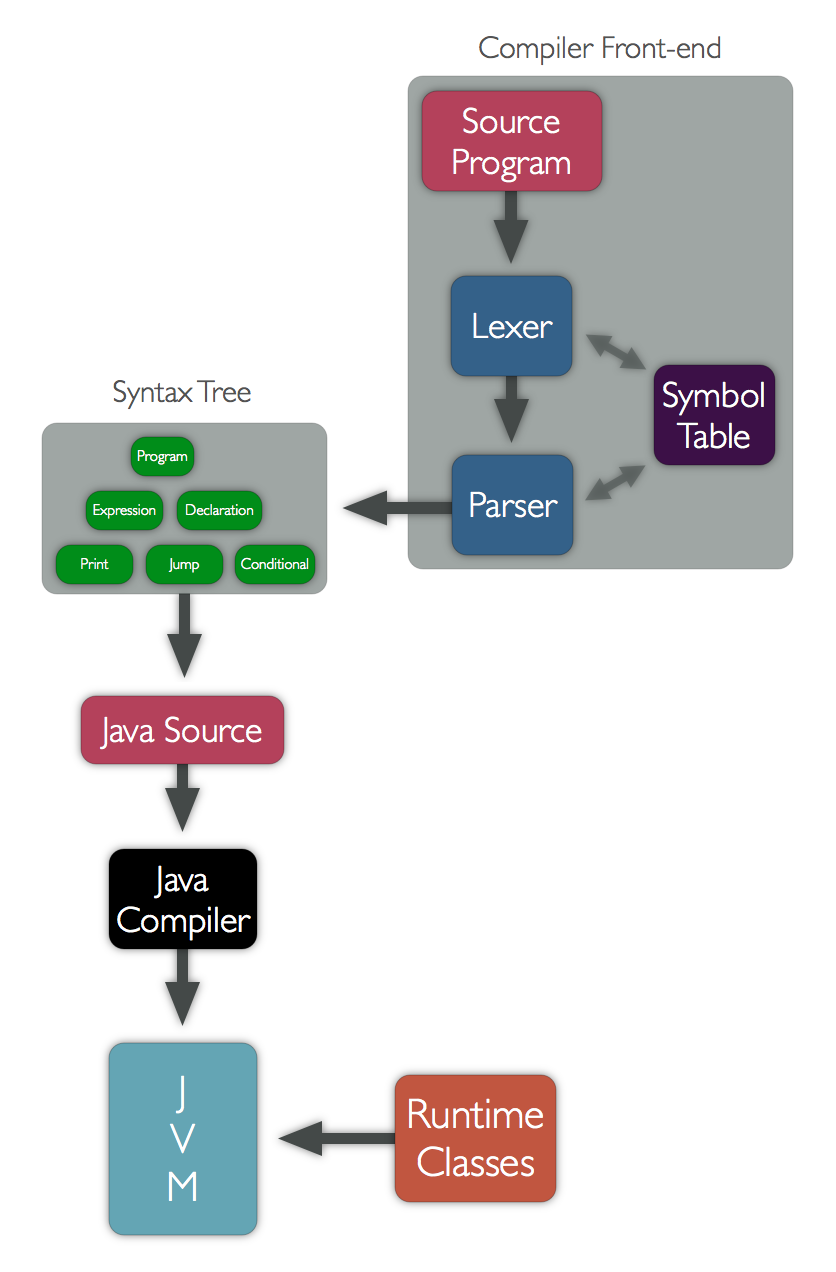
\includegraphics[scale=0.46]{blocks_scaled.png}
  \caption{Architectural Block Diagram}
  \label{blockdiagram}
\end{figure}


\section{Interfaces between Compiler Modules}\label{interfaces}
The BALL compiler's modules can be grouped into five major steps, as
enumerated below. Reference Figure \ref{blockdiagram} for a visual
representation of the interface.
\begin{enumerate}
\item First, the lexer traverses the BALL source program to be
  compiled. The lexer gathers all of the tokens, passing them to the
  parser in the same sequence. The lexer acts in a left-to-right
  method.
\item The parser then parses the sequence according to the grammar,
  matching statements. It creates a rightmost derivation, and thus
  BALL is a LR(1) language. As the parsing goes on, and the parser
  finds matches in the grammar, it adds identifiers (variables and
  functions) to the symbol table.
\item The parser outputs a syntax tree containing nodes for each
  action (actions include print statements, assignment statements,
  expressions, etc.) Every statement has a node in the syntax tree.
\item Each node generates its own Java code equivalent, checking the
  symbol table at compilation to ensure conflicts or incorrect
  declarations or calls do not exist within the code.
\item The Java code is compile by the Java compiler into bytecode. The
  Java Virtual Machine then runs this compiled bytecode as well as the
  libraries supplied in the Java backend runtime classes. These
  libraries enable BALL's syntax simplicity.
\end{enumerate}
\section{Architecture Work Distribution}
Ultimately, as was the case for all of BALL's development, work was
divided evenly, and each member contributed massively to the completed
project by being involved in every part of the process. For example,
intermediate code generation from the syntax tree was written for
different language constructs by different members of the
team. Similarly the parser and symbol table were adapted based on
which section of code a particular team member worked on at a
particular time. Often, team members worked together to solve one
particular part of the language. Thus, each module in BALL is truly a
team effort, as no particular module can be traced to one individual
person.

BALL is the ultimate baseball language. Just as baseball is a team
sport, BALL is a team-created language.

\chapter{Development Environment}\label{DevelEnv}

\section{Software Development Environment}

The software development environment that was chosen to create the
BALL compiler consists of Eclipse as the integretaged development evironment 
running on Ubuntu distribution of Linux OS. Ubuntu was chosen as the 
OS because it is open source and was readily available to all team members. 
Eclipse was chosen specifically because of its seamless integration with 
both Java and Subversion revision control system. The other tools selected
were chosen because they complemented Eclipse and Java natively.
Google Code was specially helpful in bringing everything
together since it made available to us features that were invaluable
at every stage of our compiler design. For the majority of the early
stages of our project, the record of our brainstorming sessions was
kept in a wiki stored on Google Code. This was a very helpful resource
that made it easy to trace the language and feature set
evolution. Likewise, without the ability to store our version
controlled code on Google Code, the development cycle would have been
extremely difficult to coordinate. In summary, the most important tools
used in the development of BALL were selected to leverage our team
members knowledge of Java.

\section{Software Development and Language Tools}
The Software Development tools are summarized below and illustrated in Figure \ref{toolsdiagram}

\begin{figure}[htbp]
  \centering
  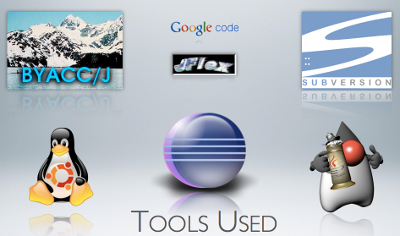
\includegraphics[scale=0.99]{softdevtools2.png}
  \caption{Tools Used}
  \label{toolsdiagram}
\end{figure}


\begin{itemize}

\item Ubuntu Linux \item Java
\item Eclipse \item Google Code
\item Subversion \item JFlex
\item BYACC/J \item Apache Ant
\item LaTeX

\end{itemize}

\section{Implementation Languages and Tools}

Java was used to develop and build our BALL compiler to leverage the
considerable expertise that our team members possessed. It was also
specially helpful that Java is highly portable and enabled our BALL
compiler to work wherever Java runs. Only Java standard libraries were
used in the creation of our compiler, to simplify and further increase
the portability of BALL. Jflex \& BYACC/J the Java flavor versions of
Lex and Yacc were used to build our lexer and parser frontend. 
Apache Ant was used to write buildfiles that automated the compilation process 
of our Java package. A bash shell script tied it all together by calling our 
BALL compiler on BALL source files, compiling the generated intermediate Java
source code, and executing the Java bytecode. Finally, LaTex was used for the 
creation of the final report to achieve a professional look and design.


\chapter{Test Plan}\label{TestPlan}
\section{Initial Testing Plan}
As a group we all felt a test driven development was crucial to bug
free code.  Test Driven Development in our case started with one line
simple grammars and simple programs.  We then would introduce small
additions to the grammar and write small programs to act as unit tests
for said additions to the grammar.  

\section{Example Test Code }
The following is a code snippet
from the unit testing program for arithmetic expressions:

\begin{singlespacing}
\begin{verbatim}

/*
 * Arithmetic Expr Test File
 */

number x, y, z;

x = 0;//x = 0
y = x + 1;//y=1
z = x / 10;//z=0

x = (z + 1) * 100; //x=100

y = z % 5 + 1;//y=1

1+2;//should get commented out in javacode
x+y;

function f1 () returns number:
    x = 13;
    return 15;
end

function f2() returns number:
    y = x * 5 % 6;
    return 2 + 4;
end

print f1() + 3;// 18
print ``f2() = `` + f2();//6
print ``x = `` + x;//13 BECAUSE ITS GLOBAL (WORLDLY)
print ``y = `` + y;//5

\end{verbatim}
\end{singlespacing}

In the code above, we extensively test arithmetic expressions.  For
instance, we check all operators on all types.  While not shown above,
testing was done intending to both successfully compile and break the
code. [A successful break is when our intended breakpoint broke and
  produced the intended error]  

\section{Test Execution}
More generally our development was very conducive to standard software
development phasing.  Initially, each member created his own testbed
where all new functionality underwent white-box and black-box testing.
Our number one rule for testing was ``never break the trunk.''  To
make sure the trunk was never broken when moving code from a sandbox
testing environment to the trunk, we always made sure at least two
people read the new code in full before importing.  Then after we
compiled the updated source code, integration testing was done.  By
doing this, we could ensure that all new components were fully
functional with all the already existing components.  Furthermore, we
could be sure that for the most part, no new bugs were introduced.
Unfortunately, some bugs did slip through to the trunk but they were
quickly squashed int the regression testing phase.  After the
previously mentioned tests were successfully completed and the
compiler was fully functional using the complete grammar, the
regression testing phase began.  Below is the code used for the first
phase of regression testing.  The code was built on initially defining
a print statement.  It then evolved to a more complex print statement.
After several more rounds of regression testing, the program evolved
to the code below.  In it, we test all the constructs outlined in the
reference manual.  It was in this phase that most of the smaller typos
and bugs were found and fixed.  For example there was a type in the
teamObj that referred to the attribute name and it should have been
upper case.  Furthermore, each step was checked to see that the
intended output was realized.  It is important to note that in this
program, accuracy was not our goal.  Accuracy testing was done only on
the more complex sim function outlined in the last part of the
language tutorial.  In that function, we noticed very accurate
predictions when testing over thousands of games.  The program output
generally similar results with small perturbation to the actual number
of wins and losses for each team.  

The programs used in the testing phases can be found in the Code
section.


\chapter{Conclusions}
\section{Lessons Learned by Team Llamamelon and Advice for Future Teams}
\subsection{Cipta Herwana, Project Manager}
\begin{itemize}
\item It's very important to keep documentation of the modules of the compiler at hand, and create them incrementally instead of creating them all after the source code is finished. Not only will the documentation better reflect the source code, but also less time will be wasted on the retracing steps.
\item Time is very important. It's a good idea to leave some days for writing up the report and updating documentation without touching the source code at all. That way, if bugs or inconsistencies with the documentation are found in the language design, there will be extra time to repair them. Similarly, it's important to do intermediate code reviews before the coding is done, for the same reasons.
\item Also on the issue of time, perhaps more important than starting early is having a clear idea of deadlines and how much time remains for each deadline. This is especially important for the project manager position, to ensure that each member of the team accomplishes their goals in a timely manner so that deadlines are met with time to spare for review.
\end{itemize}
\subsection{Daniel Lasry, Language Guru}
\begin{itemize}
\item My Java skills expanded noticeably, more so than in any other course before. Using an existing language to create a new one has definitely made me a better programmer, improving my coding skills such as commenting, optimizing, and reusing code.
\item Before working on BALL, I knew finite automata, context-free grammars, and regular expressions as a theoretical construct and had no idea when I would use them in reality. Working on this project made me understand computer science theory and its real-life applications much more.
\item Most of all, working on BALL was a great way to learn how to use tools such as SVN to work simultaneously on a single project. Each team member was able to branch off and work on their own part, merging to the trunk frequently to maintain the collaborative effort of each part of BALL. I learned a lot more about SVN than I knew before, including merging, differentiating, branching, reverting and resolving.
\end {itemize}
\subsection{Nathan Miller, System Architect}
\begin{itemize}
\item I personally love reflecting on projects to see how much I learned not only on the topic of the project itself but tangentially as well. Creating BALL enabled me to learn a lot of tools that are very exciting and interesting. These include the obvious tools like lex and yacc, but also ant, LaTeX (which I will definitely use in the future for every document I ever create), and much more.
\item In the past, teams of which I've been a part have been more like ``squads'' of people working separate of each other toward a common goal. One important thing I learned from BALL is that it's a lot better to be a cohesive group, working as one unit with smaller side coding but ultimately with everyone's fingerprints on every unit of code. 
\item Meetings are very important. It's crucial to meet with your team
  as often as possible, not only to accomplish the tasks, but to bond
  and make connections as a team. I think team connections are very
  important and here are some of the things I learned on this: Cipta
  is from Jakarta, Daniel modifies Nerf guns, Jordan has a motorcycle
  licens, and Sam is 1/8th Chinese.
\end{itemize}
\subsection{Sam Lee, System Integrator}
\begin{itemize}
\item Perhaps the most important thing that I learned is the importance of communication. It is very important to get every team member's point of view on every issue to get as many perspectives as possible. This eliminates many unforeseen problems that otherwise could derail the whole project.
\item Time management is also very important, and I learned the importance of getting a head start on large projects such as BALL in order to have steady and constant progress. Otherwise, ridiculously long meetings will happen later, causing progress to be crunched and rushed.
\item I also learned a lot about collaborative work including versioning control. Before BALL, I had very little experience with Subversion, and knew almost nothing coming into this project. Now, I have a lot more knowledge about SVN and versioning control.
\end{itemize}
\subsection{Jordan Schau, Tester/Validator}
\begin{itemize}
\item By far the most important thing I learned is the value of meeting and communication. Throughout the course of our work, our team had several long weekend meetings in which we accomplished quite a bit. Initially we were unenthusiastic about frequent meetings, but once regular meetings became commonplace, we were much more successful.
\item It is extremely important to begin working as early as possible. I cannot stress this enough. A far-off due date does not mean that it's okay to take a break, but rather that regular, steady progress should be made in order to accomplish larger goals. It was only in our last few sections that we took advantage of the time given.
\item Similarly, productivity can be a tricky thing. Generally, we were more productive as a group than by ourselves; that is, the whole is greater than the sum of its parts. I also learned that shorter, frequent meetings are more effective than infrequent marathon-length meetings.
\end{itemize}
\subsection{Team Llamamelon}
\begin{itemize}
\item Team roles should not be strictly kept.  If someone can help out
  in another area, it is extremely helpful.  Often times one of us
  would be stuck on a bug or busy and just as often a team member
  would step up and help out. Having a second, third, fourth, or even
  fifth pair of eyes looking at the same issue ensured that things
  went extremely smoothly.  Not only did this help us accomplish more
  in a short period of time but it also allowed every one of us to
  learn more about all aspects of the language and compiler.
\item It's also very important to ensure that every member of the team
  understands and is up to date on any changes. If a team member has
  to catch up on changes, this takes more time and effort than if they
  had been aware of the changes in the first place. On the other hand,
  if the whole team is up to date on the source, bugs will be solved
  and ideas will be innovated.
\item Sometimes the ideas that seem to be the best (like making BALL a
  scripting language) turn out to not be so great, but what they morph
  into (like the BALL we ended up with), if you stay dedicated, become
  infinitely more awesome, more beautiful than the original ideas!
\item We all learned quite a bit about teamwork. We would not have
  finished on time if it weren't for the amount of work and dedication
  that everyone put into the project equally and simultaneously.
\item Designing and presenting a professional project is an impressive
  and difficult thing to do. BALL is by far the largest project on
  which any of us have worked. But cooperation, placing value on
  production and cleanliness, and good organization make everything
  more efficient and easy!
\end{itemize}

\section{Suggestions for Professor Aho}
\subsection{Add}
The most helpful thing that could be added to the class would be live
demonstration of tools. If yacc/lex were demonstrated in class using
the projector, we would have had a much stronger understanding of
these tools, leading to more time spent developing our language and
less time teaching ourselves the fundamentals.
\subsection{Drop}
By far the most stressful and unnecessary part of this course is the
final exam. Because of the time-consuming nature of the final project,
none of us had a chance to fully prepare for the exam. Furthermore, it
seems to be completely unnecessary when added to the midterm, two
homework assignments, and the project. We believe the project should
be the primary focus of the class, and any other assignment should be
secondary.
\subsection{Change}
The guest lecturers were very helpful in understanding the development
of real-world languages. In addition, they were very fun and
interesting. Bjarne Stroustrup was particularly interesting, and it
would be really cool for future classes if they could also hear from
other visionaries in this field.

\pagebreak
\section{The Team}
\begin{figure}[htp]
\centering
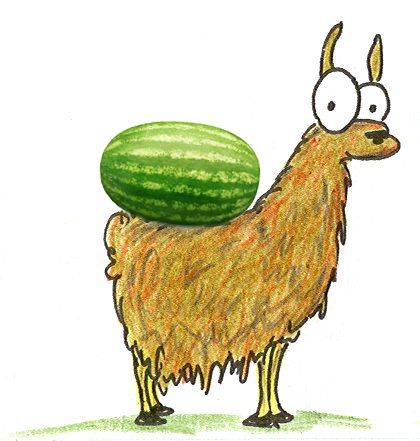
\includegraphics[scale=0.75]{lm.jpg}
\caption{Team Llamamelon, 2009}\label{llamamelon}
\end{figure}


%% <== End of hints
%%%%%%%%%%%%%%%%%%%%%%%%%%%%%%%%%%%%%%%%%%%%%%%%%%%%%%%%%%%%%

\clearpage
\chapter{Source Code}

%%%%%%
% COMPILER
%%%%%%%%
\section{compiler}

\lstinputlisting[label=ball.lex,caption=ball.lex]{../src/compiler/ball.lex}

\lstinputlisting[label=ball.y,caption=ball.y]{../src/compiler/ball.y}

\lstinputlisting[label=Run.java,caption=Run.java]{../src/compiler/Run.java}

\lstinputlisting[label=SymbolTable.java,caption=SymbolTable.java]{../src/compiler/SymbolTable.java}

%%%%%%
% CODE GENERATOR
%%%%%%%%
\section{Code Generator}

\lstinputlisting[label=ActivateStmt.java,caption=ActivateStmt.java]{../src/codegen/ActivateStmt.java}

\lstinputlisting[label=ApostrExpr.java,caption=ApostrExpr.java]{../src/codegen/ApostrExpr.java}

\lstinputlisting[label=ArithmeticExpr.java,caption=ArithmeticExpr.java]{../src/codegen/ArithmeticExpr.java}

\lstinputlisting[label=AssignmentStmt.java,caption=AssignmentStmt.java]{../src/codegen/AssignmentStmt.java}

\lstinputlisting[label=AtomicExpr.java,caption=AtomicExpr.java]{../src/codegen/AtomicExpr.java}

\lstinputlisting[label=BuiltinAttributeDef.java,caption=BuiltinAttributeDef.java]{../src/codegen/BuiltinAttributeDef.java}

\lstinputlisting[label=BuiltinFuncDef.java,caption=BuiltinFuncDef.java]{../src/codegen/BuiltinFuncDef.java}

\lstinputlisting[label=BuiltinStatDef.java,caption=BuiltinStatDef.java]{../src/codegen/BuiltinStatDef.java}

\lstinputlisting[label=BuiltinStatListDef.java,caption=BuiltinStatListDef.java]{../src/codegen/BuiltinStatListDef.java}

\lstinputlisting[label=ComparisonExpr.java,caption=ComparisonExpr.java]{../src/codegen/ComparisonExpr.java}

\lstinputlisting[label=Declaration.java,caption=Declaration.java]{../src/codegen/Declaration.java}

\lstinputlisting[label=Expr.java,caption=Expr.java]{../src/codegen/Expr.java}

\lstinputlisting[label=ExprStmt.java,caption=ExprStmt.java]{../src/codegen/ExprStmt.java}

\lstinputlisting[label=FilterExpr.java,caption=FilterExpr.java]{../src/codegen/FilterExpr.java}

\lstinputlisting[label=Funcall.java,caption=Funcall.java]{../src/codegen/Funcall.java}

\lstinputlisting[label=FuncDef.java,caption=FuncDef.java]{../src/codegen/FuncDef.java}

\lstinputlisting[label=IfStmt.java,caption=IfStmt.java]{../src/codegen/IfStmt.java}

\lstinputlisting[label=InsertionPoint.java,caption=InsertionPoint.java]{../src/codegen/InsertionPoint.java}

\lstinputlisting[label=ListInit.java,caption=ListInit.java]{../src/codegen/ListInit.java}

\lstinputlisting[label=ListType.java,caption=ListType.java]{../src/codegen/ListType.java}

\lstinputlisting[label=LogicalExpr.java,caption=LogicalExpr.java]{../src/codegen/LogicalExpr.java}

\lstinputlisting[label=MatchExpr.java,caption=MatchExpr.java]{../src/codegen/MatchExpr.java}

\lstinputlisting[label=ParseTreeNode.java,caption=ParseTreeNode.java]{../src/codegen/ParseTreeNode.java}

%\lstinputlisting[label=PlayBall.java,caption=PlayBall.java]{../src/codegen/PlayBall.java}

\lstinputlisting[label=PrintStmt.java,caption=PrintStmt.java]{../src/codegen/PrintStmt.java}

\lstinputlisting[label=Program.java,caption=Program.java]{../src/codegen/Program.java}

\lstinputlisting[label=ReturnStmt.java,caption=ReturnStmt.java]{../src/codegen/ReturnStmt.java}

\lstinputlisting[label=SimFuncDef.java,caption=SimFuncDef.java]{../src/codegen/SimFuncDef.java}

\lstinputlisting[label=StatAtom.java,caption=StatAtom.java]{../src/codegen/StatAtom.java}

\lstinputlisting[label=StatDef.java,caption=StatDef.java]{../src/codegen/StatDef.java}

\lstinputlisting[label=StatExpr.java,caption=StatExpr.java]{../src/codegen/StatExpr.java}

\lstinputlisting[label=StatMult.java,caption=StatMult.java]{../src/codegen/StatMult.java}

\lstinputlisting[label=Stmt.java,caption=Stmt.java]{../src/codegen/Stmt.java}

\lstinputlisting[label=StopdoStmt.java,caption=StopdoStmt.java]{../src/codegen/StopdoStmt.java}

\lstinputlisting[label=UnaryExpr.java,caption=UnaryExpr.java]{../src/codegen/UnaryExpr.java}

%%%%%%
% JAVA BACKEND
%%%%%%%%
\section{Java Backend}

\lstinputlisting[label=Attribute.java,caption=Attribute.java]{../src/javabackend/Attribute.java}

\lstinputlisting[label=BallDataType.java,caption=BallDataType.java]{../src/javabackend/BallDataType.java}

\lstinputlisting[label=BallList.java,caption=BallList.java]{../src/javabackend/BallList.java}

\lstinputlisting[label=Loader.java,caption=Loader.java]{../src/javabackend/Loader.java}

\lstinputlisting[label=PlayerObj.java,caption=PlayerObj.java]{../src/javabackend/PlayerObj.java}

\lstinputlisting[label=PlayerStat.java,caption=PlayerStat.java]{../src/javabackend/PlayerStat.java}

\lstinputlisting[label=SimFunction.java,caption=SimFunction.java]{../src/javabackend/SimFunction.java}

\lstinputlisting[label=Simulator.java,caption=Simulator.java]{../src/javabackend/Simulator.java}

\lstinputlisting[label=TeamAttribute.java,caption=TeamAttribute.java]{../src/javabackend/TeamAttribute.java}

\lstinputlisting[label=TeamList.java,caption=TeamList.java]{../src/javabackend/TeamList.java}

\lstinputlisting[label=TeamObj.java,caption=TeamObj.java]{../src/javabackend/TeamObj.java}

\lstinputlisting[label=TeamStat.java,caption=TeamStat.java]{../src/javabackend/TeamStat.java}

\lstinputlisting[label=Tools.java,caption=Tools.java]{../src/javabackend/Tools.java}


%%%%%%
% LEXER
%%%%%%%%
\section{Java Backend}

\lstinputlisting[label=Identifier.java,caption=Identifier.java]{../src/lexer/Identifier.java}

\lstinputlisting[label=Keyword.java,caption=Keyword.java]{../src/lexer/Keyword.java}

\lstinputlisting[label=NumericConst.java,caption=NumericConst.java]{../src/lexer/NumericConst.java}

\lstinputlisting[label=StringConst.java,caption=StringConst.java]{../src/lexer/StringConst.java}

\lstinputlisting[label=Token.java,caption=Token.java]{../src/lexer/Token.java}

\lstinputlisting[label=Type.java,caption=Type.java]{../src/lexer/Type.java}

%%%%%%
% TEST CODE
%%%%%%%%
\section{TEST CODE}

\lstinputlisting[label=testSuite.ball,caption=testSuite.ball]{../src/testSuite.ball}

\lstinputlisting[label=assign.ball,caption=assign.ball]{../src/unit_testing/assign.ball}

\lstinputlisting[label=bf.ball,caption=bf.ball]{../src/unit_testing/bf.ball}

%\lstinputlisting[label=cplx_fun.ball,caption=cplx_fun.ball]{../src/unit_testing/cplx_fun.ball}

\lstinputlisting[label=from.ball,caption=from.ball]{../src/unit_testing/from.ball}

\lstinputlisting[label=func.ball,caption=func.ball]{../src/unit_testing/func.ball}

\lstinputlisting[label=funcfail.ball,caption=funcfail.ball]{../src/unit_testing/funcfail.ball}

\lstinputlisting[label=global.ball,caption=global.ball]{../src/unit_testing/global.ball}

\lstinputlisting[label=ifstmt.ball,caption=ifstmt.ball]{../src/unit_testing/ifstmt.ball}

\lstinputlisting[label=lists.ball,caption=lists.ball]{../src/unit_testing/lists.ball}

\lstinputlisting[label=load.ball,caption=load.ball]{../src/unit_testing/load.ball}

\lstinputlisting[label=loop.ball,caption=loop.ball]{../src/unit_testing/loop.ball}

\lstinputlisting[label=play.ball,caption=play.ball]{../src/unit_testing/play.ball}

\lstinputlisting[label=s.ball,caption=s.ball]{../src/unit_testing/s.ball}

\lstinputlisting[label=simfunc.ball,caption=simfunc.ball]{../src/unit_testing/simfunc.ball}

\lstinputlisting[label=simNectar.ball,caption=simNectar.ball]{../src/unit_testing/simNectar.ball}

\lstinputlisting[label=stats.ball,caption=stats.ball]{../src/unit_testing/stats.ball}

\lstinputlisting[label=top.ball,caption=top.ball]{../src/unit_testing/top.ball}

\lstinputlisting[label=unary.ball,caption=unary.ball]{../src/unit_testing/unary.ball}

\lstinputlisting[label=where.ball,caption=where.ball]{../src/unit_testing/where.ball}



%%%%%%%%%%%%%%%%%%%%%%%%%%%%%%%%%%%%%%%%%%%%%%%%%%%%%%%%%%%%%
%% BIBLIOGRAPHY AND OTHER LISTS
%%%%%%%%%%%%%%%%%%%%%%%%%%%%%%%%%%%%%%%%%%%%%%%%%%%%%%%%%%%%%
%% A small distance to the other stuff in the table of contents (toc)
\addtocontents{toc}{\protect\vspace*{\baselineskip}}

%% The Bibliography
%% ==> You need a file 'literature.bib' for this.
%% ==> You need to run BibTeX for this (Project | Properties... | Uses BibTeX)
%\addcontentsline{toc}{chapter}{Bibliography} %'Bibliography' into toc
%\nocite{*} %Even non-cited BibTeX-Entries will be shown.
%\bibliographystyle{alpha} %Style of Bibliography: plain / apalike / amsalpha / ...
%\bibliography{literature} %You need a file 'literature.bib' for this.

%% The List of Figures
\clearpage
\addcontentsline{toc}{chapter}{List of Figures}
\listoffigures

%% The List of Tables
\clearpage
\addcontentsline{toc}{chapter}{List of Tables}
\listoftables


%%%%%%%%%%%%%%%%%%%%%%%%%%%%%%%%%%%%%%%%%%%%%%%%%%%%%%%%%%%%%
%% APPENDICES
%%%%%%%%%%%%%%%%%%%%%%%%%%%%%%%%%%%%%%%%%%%%%%%%%%%%%%%%%%%%%
\appendix
%% ==> Write your text here or include other files.

%\input{FileName} %You need a file 'FileName.tex' for this.


\end{document}

